% !TEX TS-program = pdflatex
% !TEX encoding = UTF-8 Unicode

% This is a simple template for a LaTeX document using the "article" class.
% See "book", "report", "letter" for other types of document.

\documentclass[12pt]{scrartcl} % use larger type; default would be 10pt
\usepackage[utf8]{inputenc} % set input encoding (not needed with XeLaTeX)

%%% Examples of Article customizations
% These packages are optional, depending whether you want the features they provide.
% See the LaTeX Companion or other references for full information.

%%% PAGE DIMENSIONS
\usepackage{geometry} % to change the page dimensions
\geometry{a4paper} % or letterpaper (US) or a5paper or....
% \geometry{margin=2in} % for example, change the margins to 2 inches all round
% \geometry{landscape} % set up the page for landscape
%   read geometry.pdf for detailed page layout information

% \usepackage[parfill]{parskip} % Activate to begin paragraphs with an empty line rather than an indent

%%% PACKAGES
\usepackage{booktabs} % for much better looking tables
\usepackage{array} % for better arrays (eg matrices) in maths
\usepackage{paralist} % very flexible & customisable lists (eg. enumerate/itemize, etc.)
\usepackage{verbatim} % adds environment for commenting out blocks of text & for better verbatim
\usepackage{subfig} % make it possible to include more than one captioned figure/table in a single float
%\usepackage[ngerman]{babel} % German umlauts
\usepackage[utf8]{inputenc}
\usepackage[T1]{fontenc}
\usepackage{lmodern} % fancy fonts for PDF(Reader)
\usepackage{graphicx} % show graphics
\usepackage{float} % keep images in place
\usepackage{url} %fance urls
\usepackage{nameref}
%\usepackage{subfigure} %

%%% source code listings %%%
\usepackage{listings}
\usepackage{courier}
\usepackage{color}

\definecolor{mygreen}{rgb}{0,0.6,0}
\definecolor{mygray}{rgb}{0.5,0.5,0.5}
\definecolor{mymauve}{rgb}{0.58,0,0.82}

\lstset{ %
  backgroundcolor=\color{white},   % choose the background color; you must add \usepackage{color} or \usepackage{xcolor}
  basicstyle=\footnotesize\ttfamily, % the size of the fonts that are used for the code
  breakatwhitespace=false,         % sets if automatic breaks should only happen at whitespace
  breaklines=true,                 % sets automatic line breaking
  captionpos=b,                    % sets the caption-position to bottom
  commentstyle=\color{mygreen},    % comment style
  %deletekeywords={...},            % if you want to delete keywords from the given language
  escapeinside={\%*}{*)},          % if you want to add LaTeX within your code
  extendedchars=true,              % lets you use non-ASCII characters; for 8-bits encodings only, does not work with UTF-8
  frame=single,                    % adds a frame around the code
  keepspaces=true,                 % keeps spaces in text, useful for keeping indentation of code (possibly needs columns=flexible)
  keywordstyle=\color{blue},       % keyword style
  language=Octave,                 % the language of the code
  %morekeywords={*,...},            % if you want to add more keywords to the set
  numbers=none,                    % where to put the line-numbers; possible values are (none, left, right)
  numbersep=5pt,                   % how far the line-numbers are from the code
  numberstyle=\tiny\color{mygray}, % the style that is used for the line-numbers
  rulecolor=\color{black},         % if not set, the frame-color may be changed on line-breaks within not-black text (e.g. comments (green here))
  showspaces=false,                % show spaces everywhere adding particular underscores; it overrides 'showstringspaces'
  showstringspaces=false,          % underline spaces within strings only
  showtabs=false,                  % show tabs within strings adding particular underscores
  stepnumber=2,                    % the step between two line-numbers. If it's 1, each line will be numbered
  stringstyle=\color{mymauve},     % string literal style
  tabsize=2,                       % sets default tabsize to 2 spaces
  title=\lstname                   % show the filename of files included with \lstinputlisting; also try caption instead of title
}

%%% JOBNAME %%%
\edef\Jobname{\jobname}
\catcode`\*=\active
\def*{ }
\edef\Jobname{"\scantokens\expandafter{\Jobname\noexpand}"}
\catcode`\*=12 %
%\show\Jobname

%%% HEADERS & FOOTERS
\usepackage{fancyhdr} % This should be set AFTER setting up the page geometry
\pagestyle{fancy} % options: empty , plain , fancy
\renewcommand{\headrulewidth}{0pt} % customise the layout...
\lhead{}\chead{}\rhead{
\includegraphics[scale=0.3]{./gfx/hardcodes/hardcodes-03-logo.png}}
\lfoot{\Jobname}\cfoot{}\rfoot{\thepage}
\setlength{\headheight}{65pt}

%%% SECTION TITLE APPEARANCE
\usepackage{sectsty}
\allsectionsfont{\sffamily\mdseries\upshape} % (See the fntguide.pdf for font help)
% (This matches ConTeXt defaults)

%%% ToC (table of contents) APPEARANCE
\usepackage[nottoc,notlof,notlot]{tocbibind} % Put the bibliography in the ToC
\usepackage[titles,subfigure]{tocloft} % Alter the style of the Table of Contents
\renewcommand{\cftsecfont}{\rmfamily\mdseries\upshape}
\renewcommand{\cftsecpagefont}{\rmfamily\mdseries\upshape} % No bold!

%%% PDF details %%%
\usepackage[pdftex]{hyperref}
  \hypersetup{
%%%%%%%%%%%%%%%%%%%%%%%%%%%%%%%%%%%%%%%%%%%%%%%%%%%%%% CHANGE HERE
    pdftitle={SolMan},
    pdfsubject={manual},
    pdfauthor={Sven Putze},
    pdfproducer={hardcodes.de},
    pdfkeywords={SailfishOS, Jolla, Development},
%%%%%%%%%%%%%%%%%%%%%%%%%%%%%%%%%%%%%%%%%%%%%%%%%%%%%%%%%%%%%
    pdfcreator={LaTeX},
    colorlinks,
    citecolor=black,
    filecolor=black,
    linkcolor=black,
    urlcolor=black
  }
%%% END Article customizations


\begin{document}
\begin{titlepage}
\pagenumbering{gobble}
%%%%%%%%%%%%%%%%%%%%%%%%%%%%%%%%%%%%%%%%%%%%%%%%%%%%%% CHANGE HERE
\title{Developing with SailfishOS}
\subtitle{a short introduction}
\author{Sven Putze, \url{hardcodes.de}}
% if contribution takes place and it gets a community document,
% this will be changed to represent the community efforts.
%\contactemail{mailcontact [AT] hardcodes [DOT] de}
%%%%%%%%%%%%%%%%%%%%%%%%%%%%%%%%%%%%%%%%%%%%%%%%%%%%%%%%%%%%%
%\date{} 

\maketitle
\vspace{60mm}
\begin{center}

\includegraphics[scale=0.3]{./gfx/Sailfish/sailfish-logo.png}
\end{center}
\end{titlepage}
\pagenumbering{arabic}
\setcounter{page}{1}
\tableofcontents
\pagebreak
%%%%%%%%%%%%%%%%%%%%%%%%%%%%%%%%%%%%%%%%%%%%%%%%%%%%%%%% CONTENT

\chapter{}

\section{About}

Hi, my name is Sven\cite{hc01} and I am eager to develop for the Jolla smartphone. On my way some questions came up and I tried to answer them as good as I can. After a while I decided to write down what I've learned, so that I had a central place to come back to and maybe others can benefit from this small document, too. The latest and greatest version is to be found on Github\cite{hc02}. For those who don't want to clone the git project there will be just the pdf version at \url{http://hardcodes.de/SailfishOS/Developing-with-SailfishOS.pdf}.
\\
\\
\emph{This work is licensed under the Creative Commons Attribution-NonCommercial-ShareAlike 4.0 International License. To view a copy of this license, visit \url{http://creativecommons.org/licenses/by-nc-sa/4.0/deed.en_US}.}
\\
\\
This goes only for content I have written myself, I don't claim ownership or copyright/left on cited content. Content from other parties remains under its original license.

All mentioned trademarks and trade names are the property of their respective holders, I have not marked them with a \texttrademark, \textregistered \hspace{4 pt} or \copyright \hspace{4 pt} sign. Use some common sense here. Not all information is written by myself, I've tried to quote as responsible as possible and quite intensive if appropiate. Read these notes as a human being, not like a lawyer.

If you find typos, errors or quirks, have suggestions how to make this document better, please drop me a note. Or collaborate.\hspace{4 pt}\verb,#jolla2gether,!

Don't panic if you are not comfortable with writing in \LaTeX, I am happy to use your Libre/Open Office or even Word documents.
%
\section{Download and install}\label{sec:dai}
%
You will need Virtual Box, because some components of the SailfishOS SDK come as virtual machines. Download for your development machine\cite{vbox01}.
%
\begin{figure}[H]
  \centering
  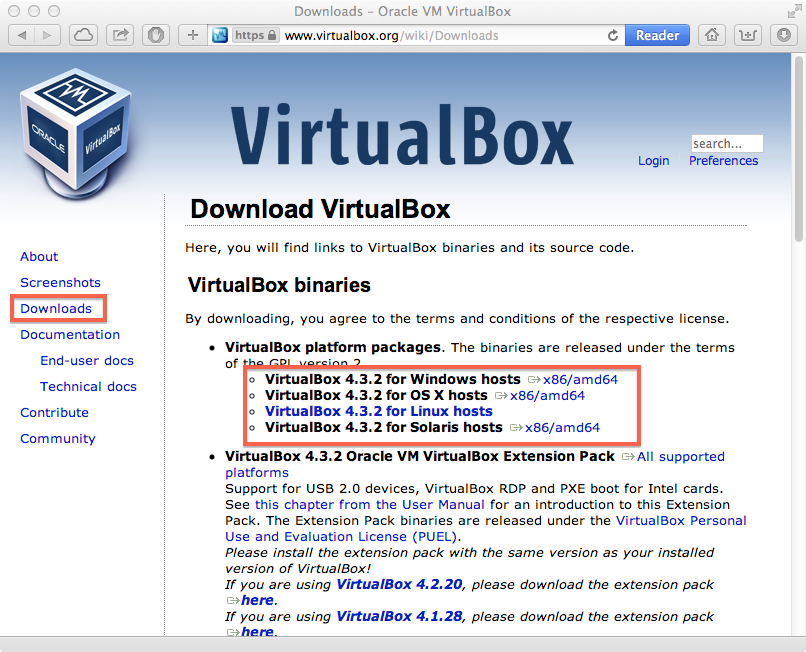
\includegraphics[scale=0.4]{./gfx/VirtualBox/vboxdownload.png} 
  \caption{Download VirtualBox from the virtualbox website.}
  \label{fig:vboxdownload}
\end{figure}
%
If you already use VirtualBox, you don't need to load it again, just skip that step. Just make sure that you have the latest updates installed.

To take a dip, head over to the Sailfish Website\cite{sailfishos01} and download the SDK for your operating system.
%
\begin{figure}[H]
  \centering
  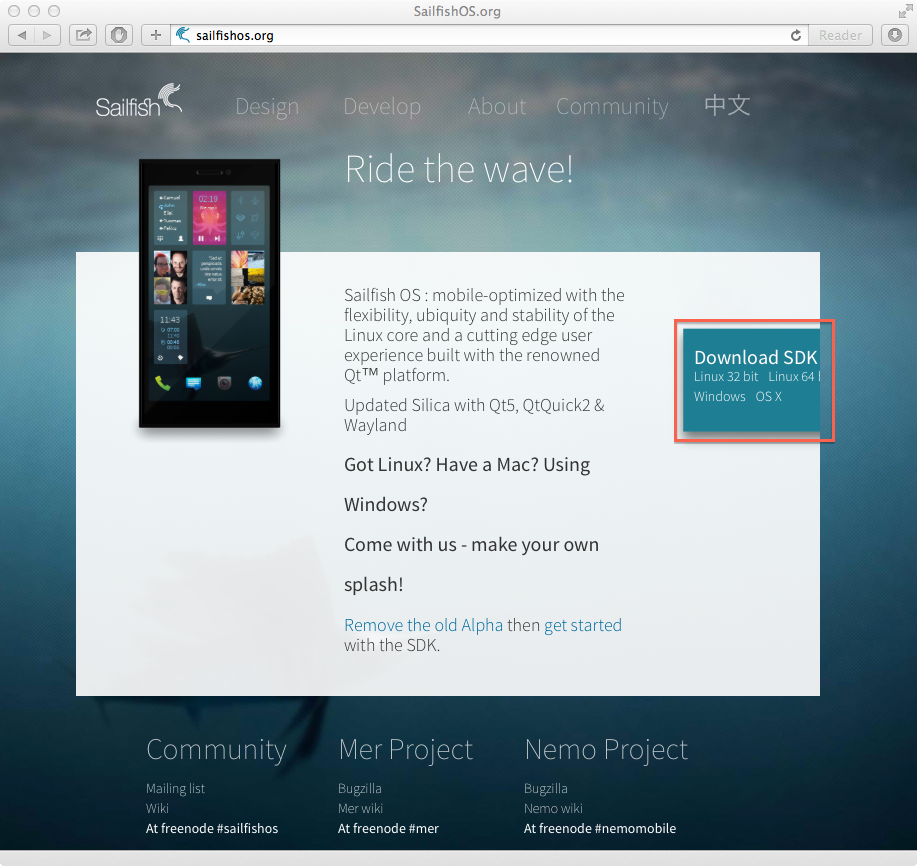
\includegraphics[scale=0.4]{./gfx/Sailfish/downloadsdk.png} 
  \caption{Download the SDK from the SailfishOS website.}
  \label{fig:downloadsdk}
\end{figure}
%
\subsection{OSX}\label{subsec:osxinstall}
%
Double click on the downloaded disk image for VirtualBox and run the installer application inside. Some file go into system folders and you must be or elevate to an admin account to install successfully.
\begin{figure}[H]
  \centering
  
\includegraphics[scale=0.2]{./gfx/OSX/osxdiskimage.png} 
  \caption{Downloaded diskimage.}
  \label{fig:osxdiskimage}
\end{figure}
%
If you use VirtualBox just for the SailfishOS SDK you don't have to care about the VirtualBox application, although you can see which folders are shared inside the preferences.

Double click on the downloaded disk image for the SailfishOS SDK and run the installer app that's inside. The installed files will end in your user directory, you don't need to be an administrator to achieve that.
%
\begin{figure}[H]
  \centering
  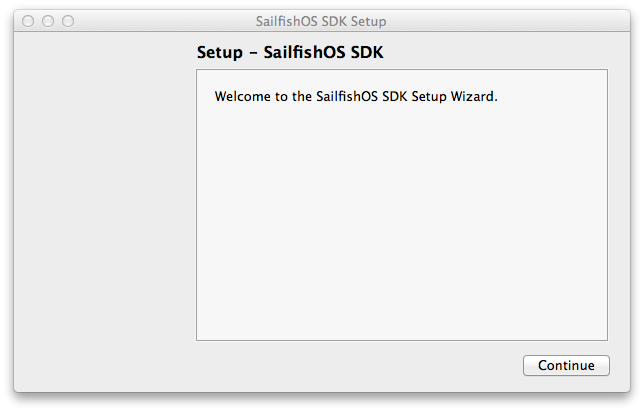
\includegraphics[scale=0.6]{./gfx/OSX/installsdk01.png} 
  \caption{Install SailfishOS SDK, step 1.}
  \label{fig:installsdk01}
\end{figure}
%
%
\begin{figure}[H]
  \centering
  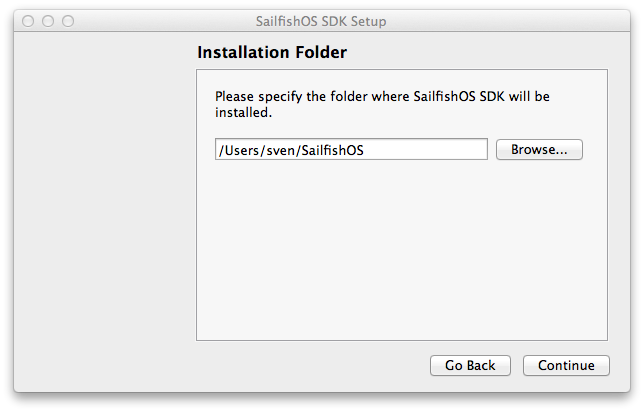
\includegraphics[scale=0.6]{./gfx/OSX/installsdk02.png} 
  \caption{Install SailfishOS SDK, step 2.}
  \label{fig:installsdk02}
\end{figure}
%
%
\begin{figure}[H]
  \centering
  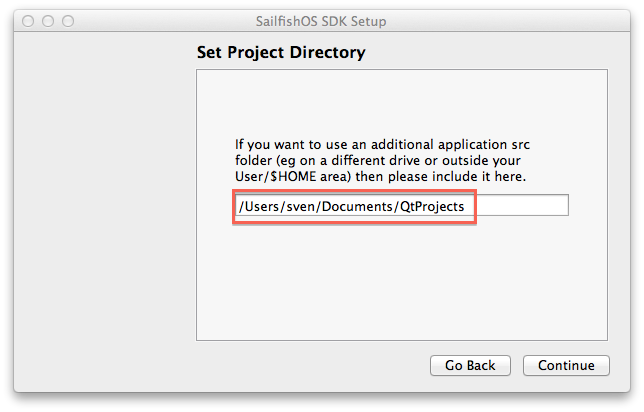
\includegraphics[scale=0.6]{./gfx/OSX/installsdk03.png} 
  \caption{Install SailfishOS SDK, step 3. Enter the path to your source code. There is no folder selector dialog, you must enter it by hand.}
  \label{fig:installsdk03}
\end{figure}
%
%
\begin{figure}[H]
  \centering
  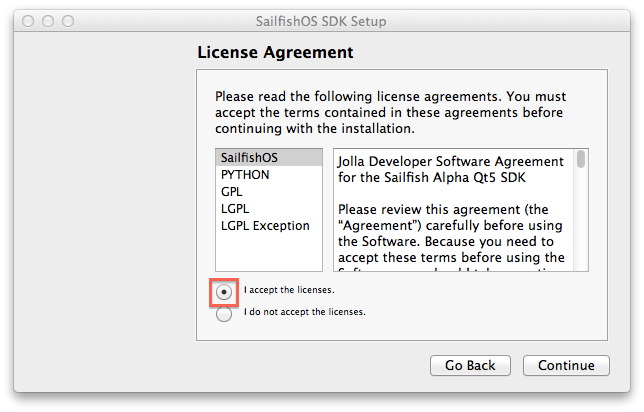
\includegraphics[scale=0.6]{./gfx/OSX/installsdk04.png} 
  \caption{Install SailfishOS SDK, step 4.}
  \label{fig:installsdk04}
\end{figure}
%
%
\begin{figure}[H]
  \centering
  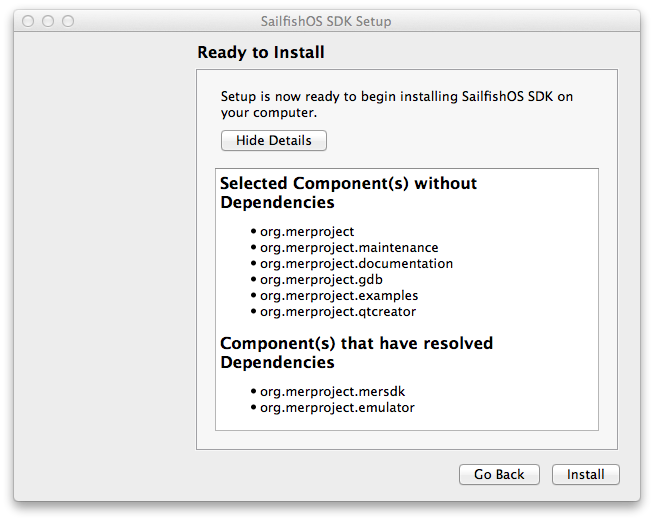
\includegraphics[scale=0.6]{./gfx/OSX/installsdk05.png} 
  \caption{Install SailfishOS SDK, step 5.}
  \label{fig:installsdk05}
\end{figure}
%
%
\begin{figure}[H]
  \centering
  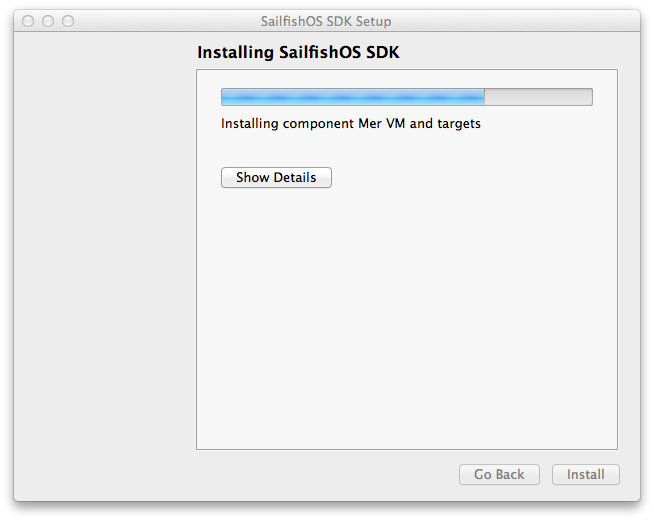
\includegraphics[scale=0.6]{./gfx/OSX/installsdk06.png} 
  \caption{Install SailfishOS SDK, step 6.}
  \label{fig:installsdk06}
\end{figure}
%
%
\begin{figure}[H]
  \centering
  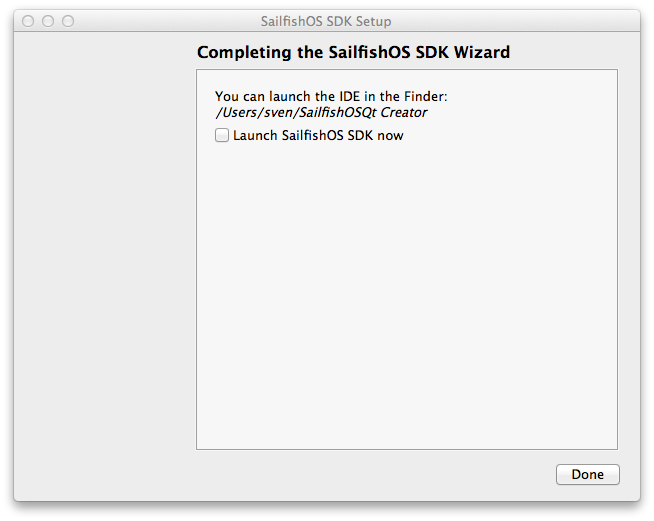
\includegraphics[scale=0.6]{./gfx/OSX/installsdk07.png} 
  \caption{Install SailfishOS SDK, step 7.}
  \label{fig:installsdk07}
\end{figure}
%
%
\begin{figure}[H]
  \centering
  
\includegraphics[scale=0.6]{./gfx/OSX/installsdk08.png} 
  \caption{Unmount SailfishOS SDK disk image, step 8.}
  \label{fig:installsdk08}
\end{figure}
%
With the installation came two hidden directories, you should know about. More about those directories will follow later on.
\\
\\
\verb,$HOME/.config/SailfishAlpha2,\\
\verb,$HOME/.scratchbox2,\\
\\
After you installed the SDK, you should immediately update the components.
%
\begin{figure}[H]
  \centering
  
\includegraphics[scale=0.6]{./gfx/QtCreator/QtCreatorUpdateNeeded.png} 
  \caption{QtCreator show that there are updates for the SDK.}
  \label{fig:QtCreatorUpdateNeeded}
\end{figure}
%
As of now the progress inside Jolla is at good pace, so it might be that there is some stuff slightly out of date in the installer (see figures \ref{fig:osxupdate} and \ref{fig:osxupdate2}).
%
\begin{figure}[H]
  \centering
  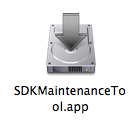
\includegraphics[scale=0.8]{./gfx/OSX/OSXSDKMaintenaceTool.png} 
  \caption{Inside the SailfishOS folder you find the maintenance application. Run it directly after the installation.}
  \label{fig:osxupdate}
\end{figure}
%
%
\begin{figure}[H]
  \centering
  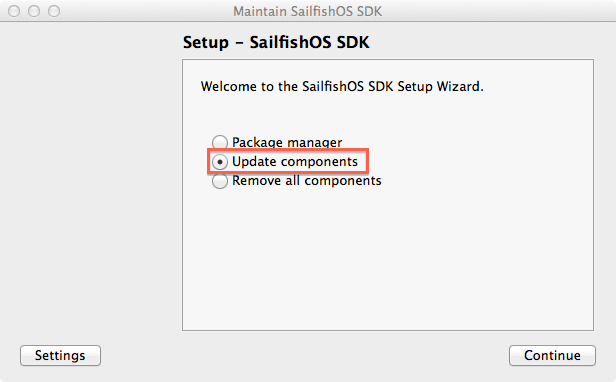
\includegraphics[scale=0.6]{./gfx/OSX/OSXSDKMaintenaceTool_run.png} 
  \caption{Update components, choose everything that is in store.}
  \label{fig:osxupdate2}
\end{figure}
%
With the SDK comes QtCreator\footnote{Look in in the "bin" folder of the SDK.}, a complete IDE for C++ development. This IDE is part of the Qt Framework\cite{qt01} and is simply reused\footnote{Customized with some little tweaks to suite the SailfishOS development.}by Jolla. Personally I use the QtCreator on my machines as well and for better differentiation I made a custom icon for the one in the SailfishOS SDK - feel free to download and use it, too\cite{hc03}.
\begin{figure}[H]
  \centering
  
\includegraphics[scale=3.0]{./gfx/Sailfish/Sailfish_Logo_Ocean.png} 
  \caption{Alternative icon for the QtCreator inside the SDK.}
  \label{fig:sdklogocustom}
\end{figure}
%
%
\subsection{Windows}
%
Double click the $\vcenter{\hbox{
\includegraphics[scale=0.6]{./gfx/VirtualBox/vboxinstaller.png}}}$ executable that you have downloaded and follow the installer.
%
\begin{figure}[H]
  \centering
  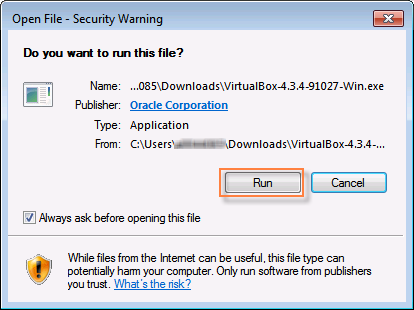
\includegraphics[scale=0.6]{./gfx/VirtualBox/vboxinstwin01.png} 
  \caption{Install VirtualBox, Step 1.}
  \label{fig:vboxinstwin01}
\end{figure}
%
%
\begin{figure}[H]
  \centering
  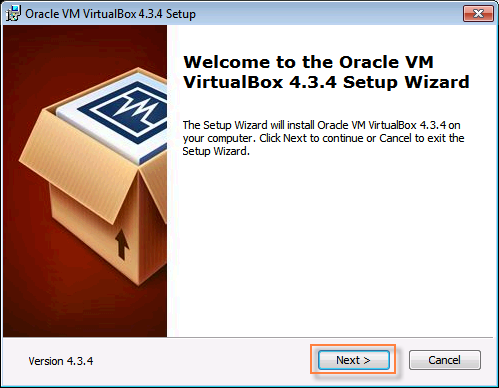
\includegraphics[scale=0.6]{./gfx/VirtualBox/vboxinstwin02.png} 
  \caption{Install VirtualBox, Step 2.}
  \label{fig:vboxinstwin02}
\end{figure}
%
%
\begin{figure}[H]
  \centering
  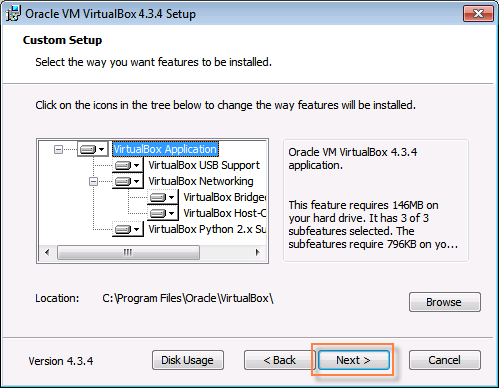
\includegraphics[scale=0.6]{./gfx/VirtualBox/vboxinstwin03.png} 
  \caption{Install VirtualBox, Step 3.}
  \label{fig:vboxinstwin03}
\end{figure}
%
\begin{figure}[H]
  \centering
  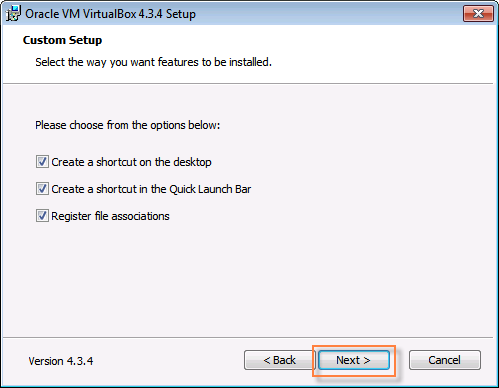
\includegraphics[scale=0.6]{./gfx/VirtualBox/vboxinstwin04.png} 
  \caption{Install VirtualBox, Step 4.}
  \label{fig:vboxinstwin01}
\end{figure}
%
\begin{figure}[H]
  \centering
  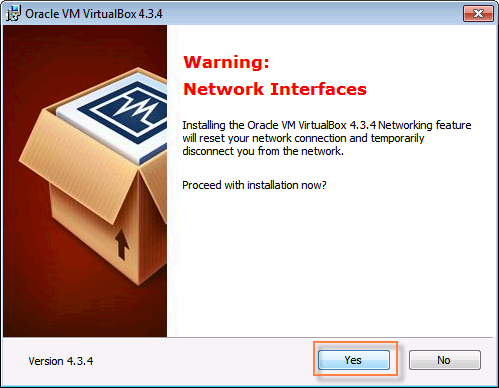
\includegraphics[scale=0.6]{./gfx/VirtualBox/vboxinstwin05.png} 
  \caption{Install VirtualBox, Step 5.}
  \label{fig:vboxinstwin05}
\end{figure}
%
\begin{figure}[H]
  \centering
  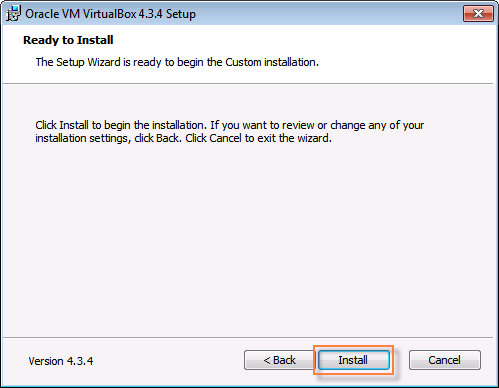
\includegraphics[scale=0.6]{./gfx/VirtualBox/vboxinstwin06.png} 
  \caption{Install VirtualBox, Step 6.}
  \label{fig:vboxinstwin06}
\end{figure}
%
\begin{figure}[H]
  \centering
  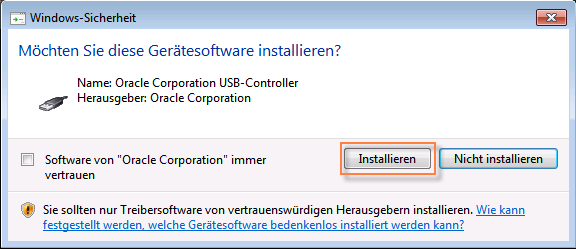
\includegraphics[scale=0.6]{./gfx/VirtualBox/vboxinstwin07.png} 
  \caption{Install VirtualBox, Step 7.}
  \label{fig:vboxinstwin07}
\end{figure}
%
\begin{figure}[H]
  \centering
  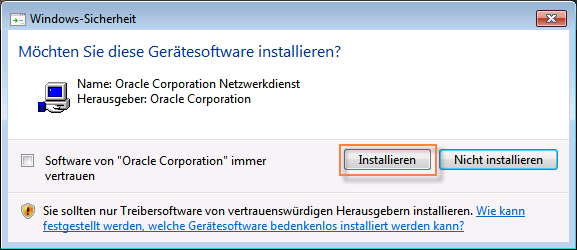
\includegraphics[scale=0.6]{./gfx/VirtualBox/vboxinstwin08.png} 
  \caption{Install VirtualBox, Step 8.}
  \label{fig:vboxinstwin08}
\end{figure}
%
\begin{figure}[H]
  \centering
  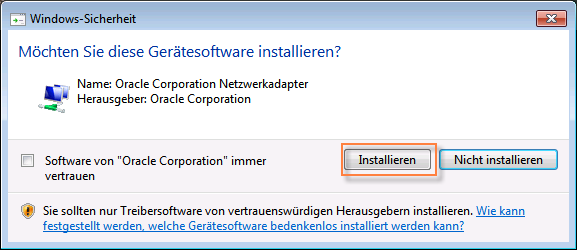
\includegraphics[scale=0.6]{./gfx/VirtualBox/vboxinstwin09.png} 
  \caption{Install VirtualBox, Step 9.}
  \label{fig:vboxinstwin09}
\end{figure}
%
\begin{figure}[H]
  \centering
  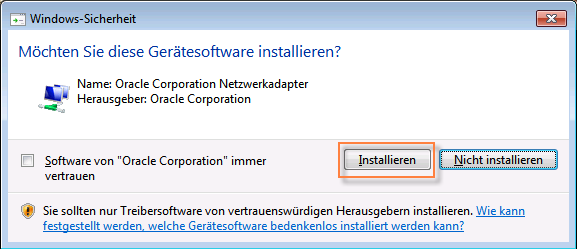
\includegraphics[scale=0.6]{./gfx/VirtualBox/vboxinstwin10.png} 
  \caption{Install VirtualBox, Step 10.}
  \label{fig:vboxinstwin10}
\end{figure}
%
\begin{figure}[H]
  \centering
  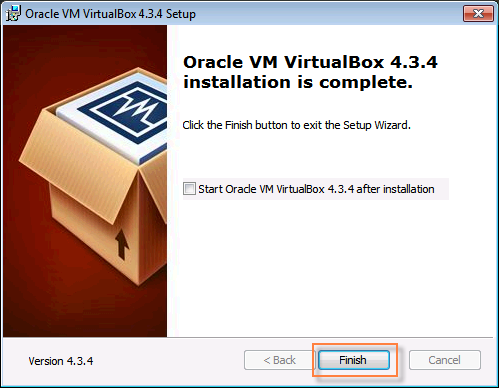
\includegraphics[scale=0.6]{./gfx/VirtualBox/vboxinstwin11.png} 
  \caption{Install VirtualBox, Step 11.}
  \label{fig:vboxinstwin11}
\end{figure}
%
Start the $\vcenter{\hbox{
\includegraphics[scale=0.6]{./gfx/Windows/sfosinstaller.png}}}$ executable and install the SDK.
%
\begin{figure}[H]
  \centering
  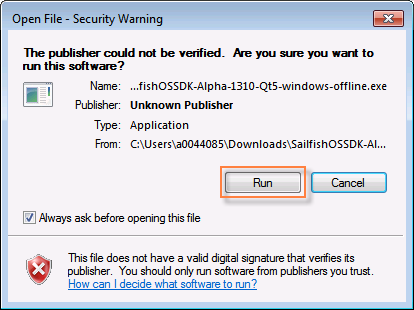
\includegraphics[scale=0.6]{./gfx/Windows/installsdkwin01.png} 
  \caption{Install SDK, Step 1.}
  \label{fig:installsdkwin01}
\end{figure}
%
\begin{figure}[H]
  \centering
  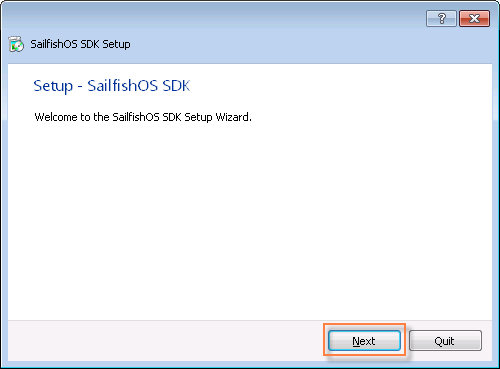
\includegraphics[scale=0.6]{./gfx/Windows/installsdkwin02.png} 
  \caption{Install SDK, Step 2.}
  \label{fig:installsdkwin02}
\end{figure}
%
\begin{figure}[H]
  \centering
  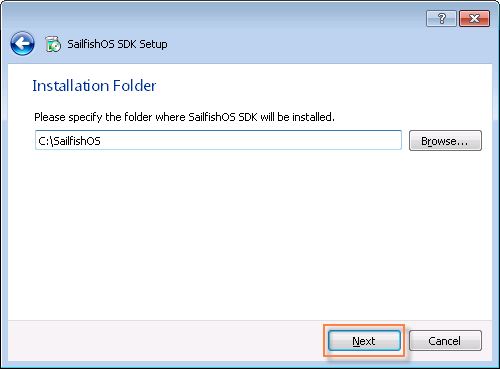
\includegraphics[scale=0.6]{./gfx/Windows/installsdkwin03.png} 
  \caption{Install SDK, Step 3.}
  \label{fig:installsdkwin03}
\end{figure}
%
\begin{figure}[H]
  \centering
  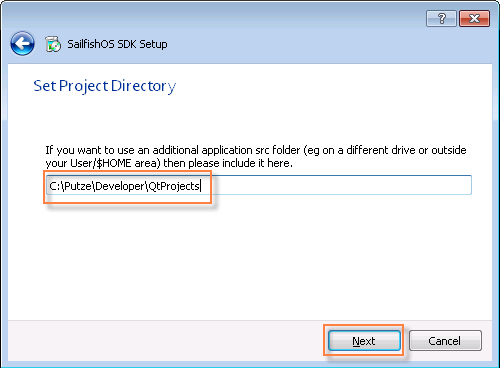
\includegraphics[scale=0.6]{./gfx/Windows/installsdkwin04.png} 
  \caption{Install SDK, Step 4.}
  \label{fig:installsdkwin04}
\end{figure}
%
\begin{figure}[H]
  \centering
  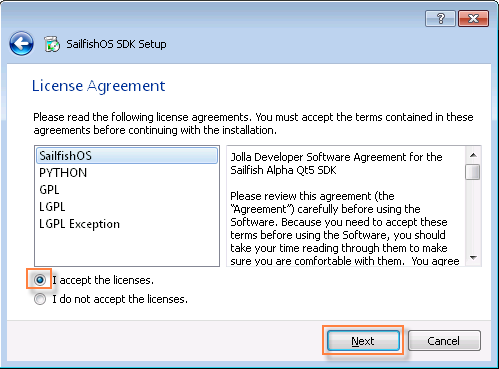
\includegraphics[scale=0.6]{./gfx/Windows/installsdkwin05.png} 
  \caption{Install SDK, Step 5.}
  \label{fig:installsdkwin05}
\end{figure}
%
\begin{figure}[H]
  \centering
  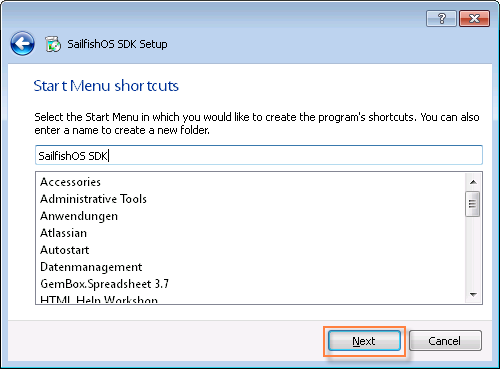
\includegraphics[scale=0.6]{./gfx/Windows/installsdkwin06.png} 
  \caption{Install VirtualBox, Step 6.}
  \label{fig:installsdkwin06}
\end{figure}
%
\begin{figure}[H]
  \centering
  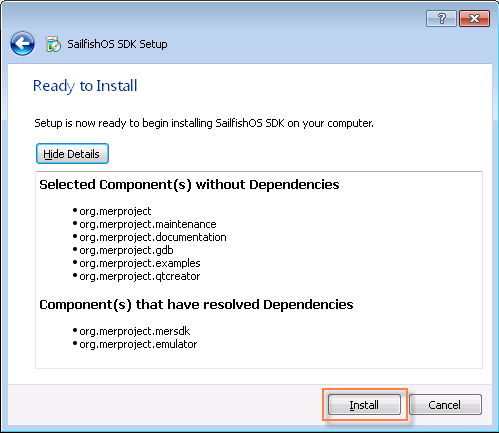
\includegraphics[scale=0.6]{./gfx/Windows/installsdkwin07.png} 
  \caption{Install VirtualBox, Step 7.}
  \label{fig:installsdkwin07}
\end{figure}
%
\begin{figure}[H]
  \centering
  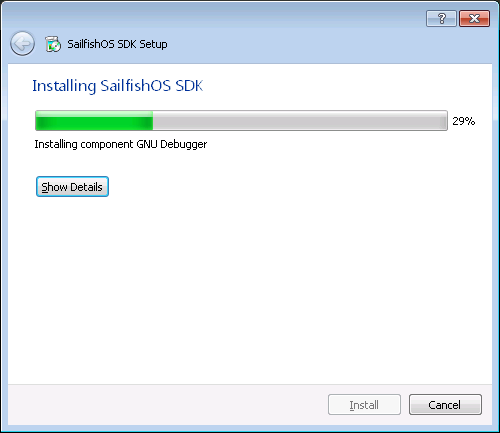
\includegraphics[scale=0.6]{./gfx/Windows/installsdkwin08.png} 
  \caption{Install VirtualBox, Step 8.}
  \label{fig:installsdkwin08}
\end{figure}
%
\begin{figure}[H]
  \centering
  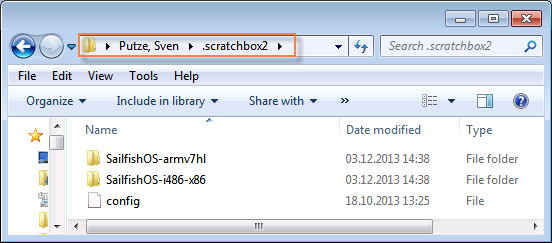
\includegraphics[scale=0.6]{./gfx/Windows/installsdkwin09.png} 
  \caption{Install VirtualBox, Step 9.}
  \label{fig:installsdkwin09}
\end{figure}
%
Start the maintenance tool from the start menu or from the SailfishOS SDK directory $\vcenter{\hbox{
\includegraphics[scale=0.8]{./gfx/Windows/sdkmaintenacetoolwin.png}}}$ and update all components.
%
\begin{figure}[H]
  \centering
  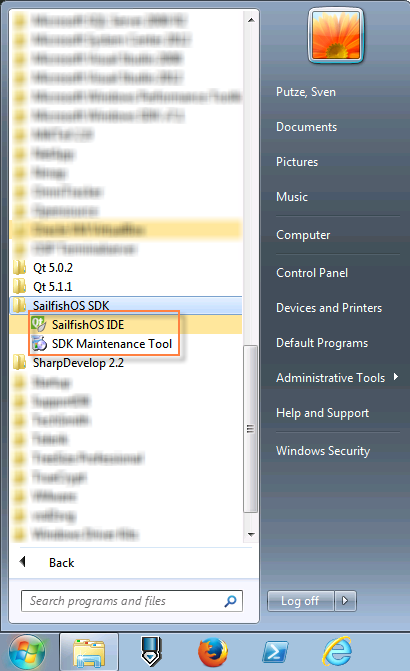
\includegraphics[scale=0.6]{./gfx/Windows/sdkwinstartmenu.png} 
  \caption{SDK and maintenance tool}
  \label{fig:sdkwinstartmenu}
\end{figure}
%
With the installation come some directories.
%
\begin{figure}[H]
  \centering
  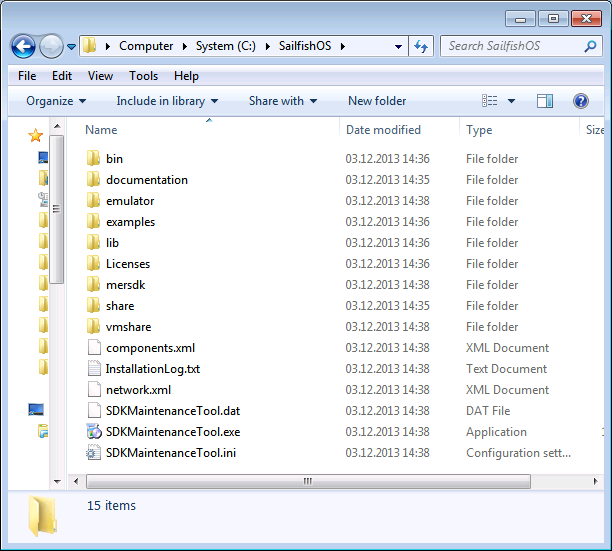
\includegraphics[scale=0.6]{./gfx/Windows/sdkdirwin01.png} 
  \caption{Directory after installation.}
  \label{fig:saddirwin01}
\end{figure}
%
%
\begin{figure}[H]
  \centering
  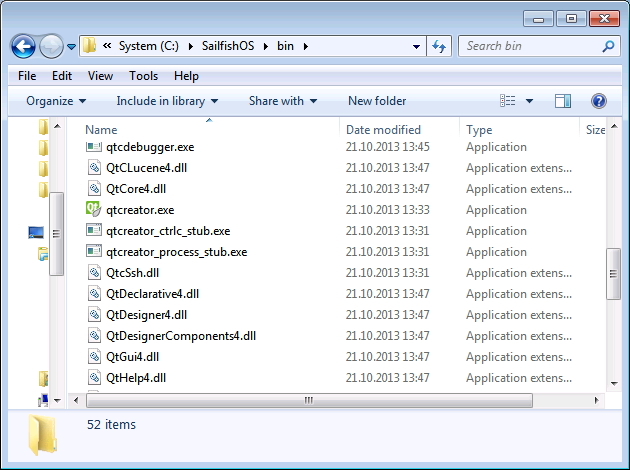
\includegraphics[scale=0.6]{./gfx/Windows/sdkdirwin02.png} 
  \caption{Directory after installation.}
  \label{fig:saddirwin02}
\end{figure}
%
%
%
\subsection{Linux}
%
Since I have not installed the SDK on Linux yet, I can not provide any information here. Sorry!

Apart from that I have no physical Linux machine that is connected to a display and can be diverted for a test installation. A virtual machine might work but that would result in VMs inside a VM, not very promising.

Volunteers present?
%
%
\subsection{Remove plugins}\label{subsec:removeplugins}
%
If you want to improve the startup time of QtCreator, you can deactivate plugins you don't need or want\footnote{On Windows and Linux the plugins should be found in Extras/Plugins.}. Just don't shoot in your foot here.
%
\begin{figure}[H]
  \centering
  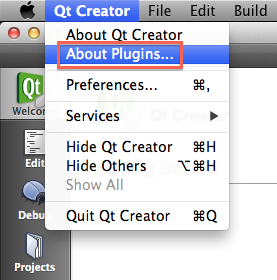
\includegraphics[scale=0.6]{./gfx/QtCreator/qtcreatorplugins.png} 
  \caption{About plugins = manage plugins.}
  \label{fig:qtcreatorplugins}
\end{figure}
%
\begin{figure}[H]
  \centering
  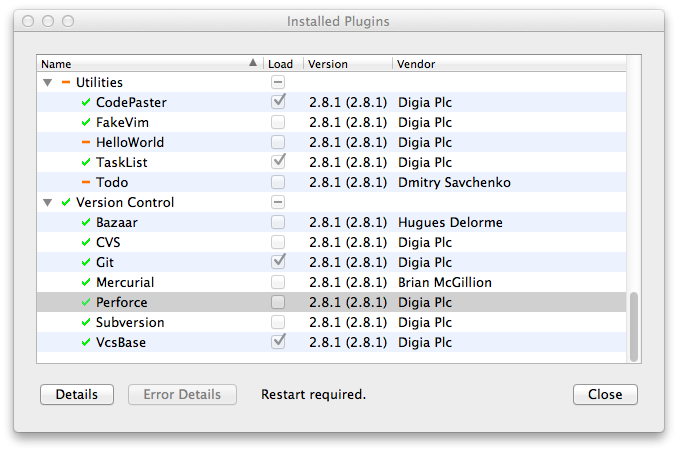
\includegraphics[scale=0.6]{./gfx/QtCreator/qtcreatordeactivateplugin.png} 
  \caption{Deactivate every plugin you don't need.}
  \label{fig:qtcreatordeactivateplugin}
\end{figure}
%
%
\section{Quickstart}\label{sec:quickstart}
%
Start the QtCreator from the fresh installed SDK.

``The SDK comes with a handy SailfishOS application template that gives you a quick way to create your very first Sailfish OS application.
Just go to File-> New File or Project in the IDE''\cite{sailfishos2}
%
\begin{figure}[H]
  \centering
  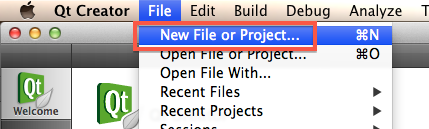
\includegraphics[scale=0.6]{./gfx/QtCreator/newsailfishproject01.png} 
  \caption{First example, step 1.}
  \label{fig:newsailfishproject01}
\end{figure}
%
%
\begin{figure}[H]
  \centering
  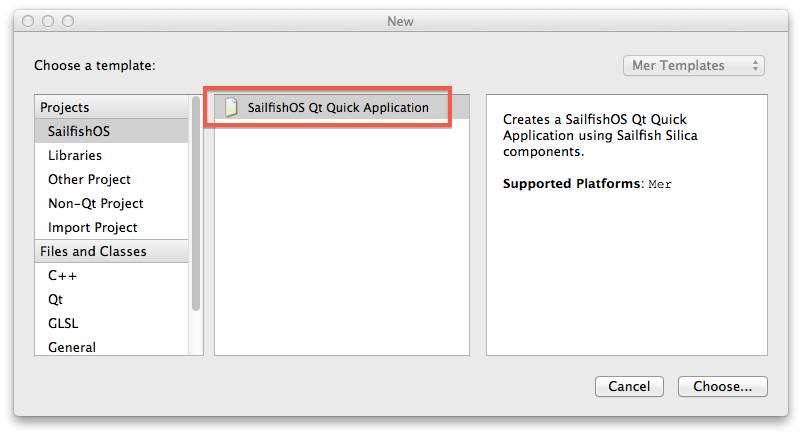
\includegraphics[scale=0.45]{./gfx/QtCreator/newsailfishproject02.png} 
  \caption{First example, step 2.}
  \label{fig:newsailfishproject02}
\end{figure}
%
%
\begin{figure}[H]
  \centering
  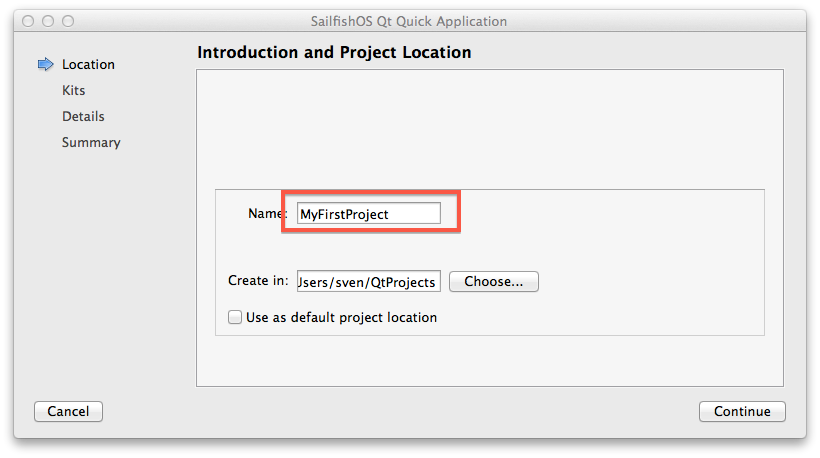
\includegraphics[scale=0.45]{./gfx/QtCreator/newsailfishproject03.png} 
  \caption{First example, step 3.}
  \label{fig:newsailfishproject03}
\end{figure}
%
%
\begin{figure}[H]
  \centering
  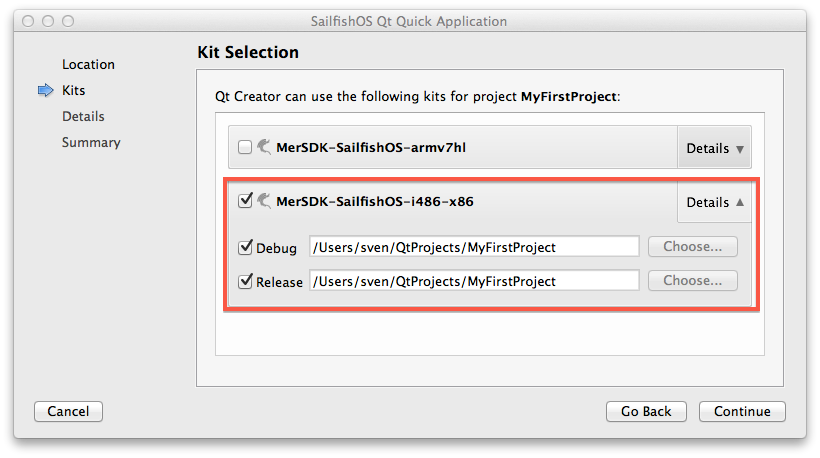
\includegraphics[scale=0.45]{./gfx/QtCreator/newsailfishproject04.png} 
  \caption{First example, step 4.}
  \label{fig:newsailfishproject04}
\end{figure}
%
%
\begin{figure}[H]
  \centering
  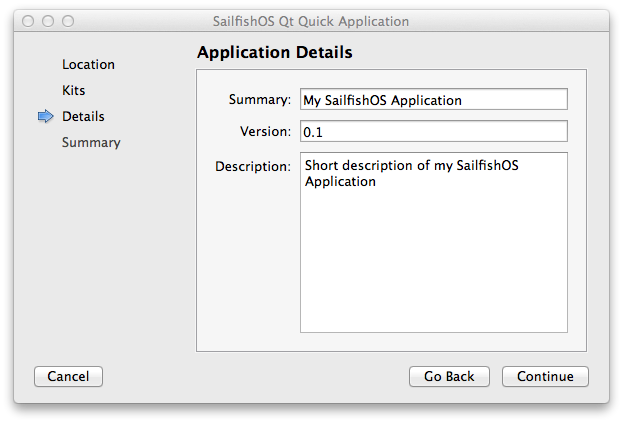
\includegraphics[scale=0.45]{./gfx/QtCreator/newsailfishproject05.png} 
  \caption{First example, step 5.}
  \label{fig:newsailfishproject05}
\end{figure}
%
%
\begin{figure}[H]
  \centering
  \includegraphics[scale=0.45]{./gfx/QtCreator/newsailfishproject06.png} 
  \caption{First example, step 1.}
  \label{fig:newsailfishproject06}
\end{figure}
%

Start the SDK from inside the QtCreator.
\begin{figure}[H]
  \centering
  \includegraphics[scale=1.0]{./gfx/QtCreator/SDKstart.png} 
  \caption{Starting the SDK.}
  \label{fig:sdkstartcreator}
\end{figure}
%
When the virtual machine with the SDK is running, apply updates if necessary. %
\begin{figure}[H]
  \centering
  \includegraphics[scale=0.4]{./gfx/QtCreator/managesdkupdate.png} 
  \caption{Updating the SDK.}
  \label{fig:managesdkupdate}
\end{figure}
%
Start the Emulator.
\begin{figure}[H]
  \centering
  \includegraphics[scale=1.0]{./gfx/QtCreator/SDKemulator.png} 
  \caption{Starting the Emulator.}
  \label{fig:emulatorstartcreator}
\end{figure}
%
Compile and run your application.
\begin{figure}[H]
  \centering
  \includegraphics[scale=1.0]{./gfx/QtCreator/runappincreator.png} 
  \caption{Build and run the application.}
  \label{fig:runappincreator}
\end{figure}
%
Easy as pie, also see figure \ref{fig:emulatorexample} on page \pageref{fig:emulatorexample}. But what happens when and where if you click on those Icons? Look in section \textit{\nameref{sec:tools}}.

A good starting point to look for a more sophisticated starting example is \emph{The missing HelloWorld. Wizard included} by Artem Marchenko\cite{gh01}. You should check that out!

And you should look in the \verb,examples, folder of the SDK of course.
%
%
\section{Know your tools}\label{sec:tools}
%
Jolla chose the Qt framework to be part of their technology stack.
``Qt is a cross-platform application and UI framework for developers using C++ or QML, a CSS \& JavaScript like language. Qt Creator is the supporting Qt IDE.
Qt, Qt Quick and the supporting tools are developed as an open source project governed by an inclusive meritocratic model. Qt can be used under open source (LGPL v2.1) or commercial terms.''\cite{qt01}

``Qt - code once, deploy everywhere'', that's the mantra of the Qt framework. If you have developed for more than one platform in the past, you know that this sounds like heaven. Maintaining different source code and technologies for each and every platform is a tedious task that can eat up all your developer resources. As if software development is not difficult enough if you stay on one platform\footnote{In my eyes software development is an art of craftsmanship and can not be done by Mr. Average and thus is a more or less complicated thing to do.}.

So there were good reasons to choose Qt as framework, no doubt about that. As of now you can develop for Android, iOS, BlackBerry and of course SailfishOS. If you look into the documentation and examples of all these platforms, you will find that those examples assume, that you are developing for this platform only. Quite stupid, if you use the Qt framework. Understandable if you think about the effort that would be necessary to build a documentation that incorporates all other possible platforms. For some time now I was wondering how I should organize my code in such a way, that allows me to develop for more than one target platform at a time. It's not just compiling for another platform! Each platform has a unique UI that behaves in an own different way, e.g. SailfishOS is gesture based, other ones are touch based.
In the long run you will create an UI for each of those targets. Period. Patterns like MVC\cite{wiki01} will come to mind, using separate business logic, yada yada.

To cut a long story short, why am I writing about this stuff, this section is supposed to be about tools? When you prepare a software project for the use for more than one target platform, you will start organizing stuff differently. Maybe you use folders that have the name of the targets to differentiate stuff that's platform dependent. Maybe you even create a business logic that is really unique and capsulated in such clever way that it can be reused and does not know anything about the outside world. Such a business logic or model can be driven from tests, command line tools, web or different native UIs. Would be nice to have it in a separate folder or even subproject. If you start to move and/or rename things, your tools will break. Intentionally.

By examining those fractures you can learn a lot about your tools that otherwise work so silently in the background. So go on and break your tools!\footnote{Ok, not so short :-)}

Here is what I've learned so far.
%
\subsection{Technology stack}
%
\begin{figure}[H]
  \centering
  \includegraphics[scale=0.8]{./gfx/Sailfish/Sailfish_Architecture.png} 
  \caption{Sailfish architecture, taken from\\https://sailfishos.org/images/Sailfish\_Architecture.png.}
  \label{fig:SailfishArchitecture}
\end{figure}
%
\subsection{QtCreator integrated development environment (IDE)}\label{subset:QtCreator}
%
``QtCreator is a cross platform integrated development environment (IDE) tailored to the needs of Qt developers. It has been extended to add support for Sailfish UI application development using Sailfish Silica components. It provides a sophisticated code editor with version control, project and build management system integration.''\cite{sailfishos3}.

Reusing an existing open source IDE is a smart move from Jolla. Why should they waste resources on developing something that has already done by others? Or why should they burn up their staff for all those development solutions out there? Be it Visual Studio, Eclipse, Emacs or even Vi. If you really dive in the tools, you can also use those but I doubt that Jolla will provide you with support if something does not work. Working with QtCreator is also quite natural in the Qt universe albeit being a fast IDE. So have a look in the preferences\footnote{On Windows and Linux they should be found in Extras/Options.}.
\begin{figure}[H]
  \centering
  \includegraphics[scale=0.7]{./gfx/QtCreator/QtCreatorPreferences.png} 
  \caption{Open the QtCreator preferences.}
  \label{fig:creatorpref}
\end{figure}
%
I will not walk through every setting of QtCreator, \cite{qt02} is a better place to start for basic questions.
Also I will not use the order of tabs in the preferences, but try to follow the sequence in which those tools touch your source code.
%
%
\subsubsection{kits}\label{subsubsec:kits}
%
But before we do that, we must talk about \textit{kits}. A kit is kind of an umbrella setting, which combines the information of the following bits and pieces, like \verb,qmake,, \verb,compiler,, and \verb,device type,. This is the information hub that QtCreator uses to pull all information together and initiate its actions.
\begin{figure}[H]
  \centering
  \includegraphics[scale=0.35]{./gfx/QtCreator/kits486.png} 
  \caption{Preferences, kits tab.}
  \label{fig:creatorkits}
\end{figure}
%
%
\subsubsection{qmake}\label{subsubsec:qmake}
%
\begin{figure}[H]
  \centering
  \includegraphics[scale=0.35]{./gfx/QtCreator/QtCreatorQtVersions.png} 
  \caption{Preferences, QtVersions tab.}
  \label{fig:qmake486pref}
\end{figure}
%
``qmake is a tool that helps simplify the build process for development project across different platforms. qmake automates the generation of Makefiles so that only a few lines of information are needed to create each Makefile. qmake can be used for any software project, whether it is written in Qt or not.
qmake generates a Makefile based on the information in a project file. Project files are created by the developer, and are usually simple, but more sophisticated project files can be created for complex projects. qmake contains additional features to support development with Qt, automatically including build rules for moc and uic. qmake can also generate projects for Microsoft Visual studio without requiring the developer to change the project file.''\cite{qt03}
%
\begin{figure}[H]
  \centering
  \includegraphics[scale=0.45]{./gfx/QtCreator/qmakedetails.png} 
  \caption{Preferences, QtVersions tab., qmake details}
  \label{fig:qmakedetailspref}
\end{figure}
%
UIC is a tool that creates C++ classes from XML information generated with the UI designer inside QtCreator. This designer is for Qt widgets which should not be used with SailfishOS and is not further explained in this document.

MOC is the Meta-Object Compiler which ``reads a C++ header file. If it finds one or more class declarations that contain the \verb,Q_OBJECT, macro, it produces a C++ source file containing the meta-object code for those classes.''\cite{qt04}. If you use \verb,qmake, to produce your Makefile, you don't have to worry about it, the rules are created automatically.
%
\begin{figure}[H]
  \centering
  \includegraphics[scale=0.6]{./gfx/bash/qmake486.png} 
  \caption{Running qmake from command line.}
  \label{fig:qmake486commandline}
\end{figure}
%
If you run qmake manually, you will find out that it tries to connect to the \textit{Mer build engine for cross compilation}. The error also appears if the virtual machine is up and running. In the Projects settings you can see how \verb,qmake, is invoked if started by QtCreator.
%
\begin{figure}[H]
  \centering
  \includegraphics[scale=0.8]{./gfx/QtCreator/projects.png} 
  \caption{Project settings.}
  \label{fig:qmakeprojectsettings}
\end{figure}
%
%
\begin{figure}[H]
  \centering
  \includegraphics[scale=0.5]{./gfx/QtCreator/buildstepsqmake.png} 
  \caption{Build steps for qmake.}
  \label{fig:qmakebuildsteps}
\end{figure}
%
Using those parameters via command line does not work, too.
\begin{figure}[H]
  \centering
  \includegraphics[scale=0.6]{./gfx/bash/qmakewithparam.png} 
  \caption{Running qmake from command line with parameters from build steps.}
  \label{fig:qmake486buildstepsparamcommandline}
\end{figure}
%
If \verb,qmake, is invoked by the QtCreator it works just fine.
\begin{figure}[H]
  \centering
  \includegraphics[scale=0.5]{./gfx/QtCreator/qmakerunfromqtcreator.png} 
  \caption{Running qmake from QtCreator (Build menu).}
  \label{fig:qmake486runfromqtcreator}
\end{figure}
%
As a result you will find a \verb,Makefile, in your project directory.
\begin{figure}[H]
  \centering
  \includegraphics[scale=0.5]{./gfx/QtCreator/qmakeresult.png} 
  \caption{Result of running qmake from QtCreator (Build menu).}
  \label{fig:qmake486result}
\end{figure}
%
Here is the snippet about the MOC.
%
\begin{lstlisting}[language=make]
####### Sub-libraries

distclean: clean
	-$(DEL_FILE) $(TARGET) 
	-$(DEL_FILE) Makefile


mocclean: compiler_moc_header_clean compiler_moc_source_clean

mocables: compiler_moc_header_make_all compiler_moc_source_make_all

check: first

compiler_rcc_make_all:
compiler_rcc_clean:
compiler_wayland-server-header_make_all:
compiler_wayland-server-header_clean:
compiler_wayland-client-header_make_all:
compiler_wayland-client-header_clean:
compiler_qtwayland-client-header_make_all:
compiler_qtwayland-client-header_clean:
compiler_qtwayland-server-header_make_all:
compiler_qtwayland-server-header_clean:
compiler_moc_header_make_all: moc/moc_qbusinesslogic.cpp
compiler_moc_header_clean:
	-$(DEL_FILE) moc/moc_qbusinesslogic.cpp
moc/moc_qbusinesslogic.cpp: /usr/include/qt5/QtCore/QObject \
		/usr/include/qt5/QtCore/qobject.h \
		/usr/include/qt5/QtCore/qobjectdefs.h \
		/usr/include/qt5/QtCore/qnamespace.h \
		/usr/include/qt5/QtCore/qglobal.h \
		/usr/include/qt5/QtCore/qconfig.h \
		/usr/include/qt5/QtCore/qfeatures.h \
		/usr/include/qt5/QtCore/qsystemdetection.h \
		/usr/include/qt5/QtCore/qcompilerdetection.h \
		/usr/include/qt5/QtCore/qprocessordetection.h \
		/usr/include/qt5/QtCore/qglobalstatic.h \
		/usr/include/qt5/QtCore/qatomic.h \
		/usr/include/qt5/QtCore/qbasicatomic.h \
		/usr/include/qt5/QtCore/qatomic_bootstrap.h \
		/usr/include/qt5/QtCore/qgenericatomic.h \
		/usr/include/qt5/QtCore/qatomic_msvc.h \
		/usr/include/qt5/QtCore/qatomic_integrity.h \
		/usr/include/qt5/QtCore/qoldbasicatomic.h \
		/usr/include/qt5/QtCore/qatomic_vxworks.h \
		/usr/include/qt5/QtCore/qatomic_power.h \
		/usr/include/qt5/QtCore/qatomic_alpha.h \
		/usr/include/qt5/QtCore/qatomic_armv7.h \
		/usr/include/qt5/QtCore/qatomic_armv6.h \
		/usr/include/qt5/QtCore/qatomic_armv5.h \
		/usr/include/qt5/QtCore/qatomic_bfin.h \
		/usr/include/qt5/QtCore/qatomic_ia64.h \
		/usr/include/qt5/QtCore/qatomic_mips.h \
		/usr/include/qt5/QtCore/qatomic_s390.h \
		/usr/include/qt5/QtCore/qatomic_sh4a.h \
		/usr/include/qt5/QtCore/qatomic_sparc.h \
		/usr/include/qt5/QtCore/qatomic_x86.h \
		/usr/include/qt5/QtCore/qatomic_cxx11.h \
		/usr/include/qt5/QtCore/qatomic_gcc.h \
		/usr/include/qt5/QtCore/qatomic_unix.h \
		/usr/include/qt5/QtCore/qmutex.h \
		/usr/include/qt5/QtCore/qlogging.h \
		/usr/include/qt5/QtCore/qflags.h \
		/usr/include/qt5/QtCore/qtypeinfo.h \
		/usr/include/qt5/QtCore/qtypetraits.h \
		/usr/include/qt5/QtCore/qsysinfo.h \
		/usr/include/qt5/QtCore/qobjectdefs_impl.h \
		/usr/include/qt5/QtCore/qstring.h \
		/usr/include/qt5/QtCore/qchar.h \
		/usr/include/qt5/QtCore/qbytearray.h \
		/usr/include/qt5/QtCore/qrefcount.h \
		/usr/include/qt5/QtCore/qarraydata.h \
		/usr/include/qt5/QtCore/qstringbuilder.h \
		/usr/include/qt5/QtCore/qlist.h \
		/usr/include/qt5/QtCore/qalgorithms.h \
		/usr/include/qt5/QtCore/qiterator.h \
		/usr/include/qt5/QtCore/qcoreevent.h \
		/usr/include/qt5/QtCore/qscopedpointer.h \
		/usr/include/qt5/QtCore/qmetatype.h \
		/usr/include/qt5/QtCore/qvarlengtharray.h \
		/usr/include/qt5/QtCore/qcontainerfwd.h \
		/usr/include/qt5/QtCore/qisenum.h \
		/usr/include/qt5/QtCore/qobject_impl.h \
		model/qt/qbusinesslogic.h
	/usr/lib/qt5/bin/moc $(DEFINES) $(INCPATH) -I/usr/lib/gcc/i486-meego-linux/4.6.4/../../../../include/c++/4.6.4 -I/usr/lib/gcc/i486-meego-linux/4.6.4/../../../../include/c++/4.6.4/i486-meego-linux -I/usr/lib/gcc/i486-meego-linux/4.6.4/../../../../include/c++/4.6.4/backward -I/usr/lib/gcc/i486-meego-linux/4.6.4/include -I/usr/local/include -I/usr/include model/qt/qbusinesslogic.h -o moc/moc_qbusinesslogic.cpp
\end{lstlisting}
%
The \verb,qmake, from the SailfishOS SDK is just a simple bash script, that invokes \verb,merssh,.
%
\begin{lstlisting}[language=bash]
#!/bin/bash
exec "/Users/sven/SailfishOS/bin/Qt Creator.app/Contents/MacOS/../Resources/merssh" -sdktoolsdir "/Users/sven/.config/SailfishAlpha2/mer-sdk-tools/MerSDK" -commandtype mb2 -mertarget SailfishOS-i486-x86 qmake $@oluhuone:SailfishOS-i486-x86
\end{lstlisting}
%
So that's the trick: \verb,$@, is replaced with the \verb,qmake, call parameters, \verb,oluhuone, is just the name of one of my computers.
%
%
\subsubsection{.pro file}
%
Project files contain all the information required by \nameref{subsubsec:qmake} to build your application, library, or plugin. Generally, you use a series of declarations to specify the resources in the project, but support for simple programming constructs enables you to describe different build processes for different platforms and environments[QtCreator help].

If you select the help mode of QtCreator and switch to \emph{Index}, you can search amongst other things for \verb,qmake, and have a look at the \verb,qmake Variable Reference,.
%
\begin{figure}[H]
  \centering
  \includegraphics[scale=0.7]{./gfx/QtCreator/HelpSelectIndex.png} 
  \caption{QtCreator, Help, Index.}
  \label{fig:HelpSelectIndex}
\end{figure}
%
The fundamental behavior of qmake is influenced by variable declarations that define the build process of each project. Some of these declare resources, such as headers and source files, that are common to each platform. Others are used to customize the behavior of compilers and linkers on specific platforms[QtCreator help].
%
\begin{figure}[H]
  \centering
  \includegraphics[scale=0.7]{./gfx/QtCreator/HelpSearchQmake.png} 
  \caption{QtCreator, search for qmake.}
  \label{fig:HelpSearchQmake}
\end{figure}
%
%
\subsubsection{merssh}\label{subsubsec:merssh}
%
Looking with \verb,top, showed a process called \verb,merssh, when \verb,qmake, was started via QtCreator. Interesting, what's that?
%
\begin{figure}[H]
  \centering
  \includegraphics[scale=0.6]{./gfx/bash/merssh.png} 
  \caption{What is merssh?.}
  \label{fig:merssh}
\end{figure}
%
So it is part of the QtCreator that is shipped with the SailfishOS SDK.
%
\begin{figure}[H]
  \centering
  \includegraphics[scale=0.6]{./gfx/bash/mersshinvoked.png} 
  \caption{merssh invoked, what's it?.}
  \label{fig:mersshinvoked}
\end{figure}
%
All the programs called by QtCreator during the build and run process are more or less just proxy scripts\footnote{OSX and Linux come with bash scripts, Windows comes with?} that call \verb,merssh,, which in turn calls something on the \nameref{subsec:MerSDK}, see page \pageref{subsec:MerSDK}.

More than that, it calls \verb,sb2, which is short for Scratchbox2, have a look at section \nameref{subsec:scratchbox2} on page \pageref{subsec:scratchbox2}, there are more details. For now let's just assume that ``Scratchbox 2 is a cross-compilation engine, it can be used to create a highly flexible SDK.''\cite{sb2}.
%
\begin{figure}[H]
  \centering
  \includegraphics[scale=0.5]{./gfx/QtCreator/merplugin.png} 
  \caption{Mer plugin, maybe that's the source of merssh?.}
  \label{fig:merplugin}
\end{figure}
%
I've grepped the command line for the \verb,merssh,
\begin{lstlisting}[language=bash]
$ ps -ef|grep "merssh"
\end{lstlisting}
%
And the result is:
\begin{lstlisting}[language=bash]
/Users/sven/SailfishOS/bin/Qt Creator.app/Contents/MacOS/../Resources/merssh -sdktoolsdir /Users/sven/.config/SailfishAlpha2/mer-sdk-tools/MerSDK -commandtype mb2 -mertarget SailfishOS-i486-x86 qmake /Users/sven/QtProjects/TestSailfishOS/TestSailfishOS.pro -r -spec linux-g++ CONFIG+=debug CONFIG+=declarative_debug CONFIG+=qml_debug -after OBJECTS_DIR=obj MOC_DIR=moc UI_DIR=ui RCC_DIR=rcc
\end{lstlisting}
%
The picture is getting clearer now. QtCreator starts the SDK version of \verb,qmake, which call \verb,merssh, with all parameters needed to call \verb,qmake, via \verb,mb2, on the virtual machine.
%
%
\subsubsection{gcc}\label{subsubsec:compilers:gcc}
%
%
\begin{figure}[H]
  \centering
  \includegraphics[scale=0.35]{./gfx/QtCreator/Compilers.png} 
  \caption{Preferences, compiler tab.}
  \label{fig:creatorcompilers}
\end{figure}
%
The SailfishOS SDK uses GCC as compiler. It is run inside the \nameref{subsec:MerSDK}, see page \pageref{subsec:MerSDK}. Stored on your development machine is only a stub or proxy that wants to connect to the virtual machine and start compiling from there.
%
\begin{figure}[H]
  \centering
  \includegraphics[scale=0.6]{./gfx/bash/gcc486.png} 
  \caption{Running GCC from command line.}
  \label{fig:gcc486commandline}
\end{figure}
%
So far I don't know why this piece of software is not installed with the rest of the SDK, \verb, ~/.config, is not a directory where I would expect executables. The error message even shows up if the \textit{Mer build engine for cross compilation} is up and running. Again this helper program is invoked via \nameref{subsubsec:merssh}, see page \pageref{subsubsec:merssh}.

Looking inside \verb,gcc, from the SDK I also find a bash script:
\begin{lstlisting}[language=bash]
#!/bin/bash
exec "/Users/sven/SailfishOS/bin/Qt Creator.app/Contents/MacOS/../Resources/merssh" -sdktoolsdir "/Users/sven/.config/SailfishAlpha2/mer-sdk-tools/MerSDK" -commandtype sb2 -mertarget SailfishOS-i486-x86 gcc $@oluhuone:SailfishOS-i486-x86
\end{lstlisting}
%
\verb,$@, is replaced with the \verb,gcc, call parameters, \verb,oluhuone, is just the name of my current machine.

One questions remains: when is this ever called? To my understanding \verb,qmake, and \verb,make, are called on the \nameref{subsec:MerSDK}. I would conclude that the compiler is invoked from inside the VM.
%
%
\subsubsection{make}\label{subsubsec:make}
%
Again, \verb,make, is just a bash script, \verb,$@, replaced, \verb,oluhuone, my machine:
%
\begin{lstlisting}[language=bash]
#!/bin/bash
exec "/Users/sven/SailfishOS/bin/Qt Creator.app/Contents/MacOS/../Resources/merssh" -sdktoolsdir "/Users/sven/.config/SailfishAlpha2/mer-sdk-tools/MerSDK" -commandtype mb2 -mertarget SailfishOS-i486-x86 make $@oluhuone:SailfishOS-i486-x86
\end{lstlisting}
%
%
I've grepped the command line for the \verb,merssh, while building the application.
%
\begin{lstlisting}[language=bash]
$ ps -ef|grep "merssh"
\end{lstlisting}
%
Resulting in
%
\begin{lstlisting}[language=bash]
/Users/sven/SailfishOS/bin/Qt Creator.app/Contents/MacOS/../Resources/merssh -sdktoolsdir /Users/sven/.config/SailfishAlpha2/mer-sdk-tools/MerSDK -commandtype mb2 -mertarget SailfishOS-i486-x86 make
\end{lstlisting}
%
Calling \verb,make, on the development machine just calls a proxy script, which forwards the command via \verb,merssh, and executes \verb,make, on the \nameref{subsec:MerSDK}.
%
%
\subsubsection{rpm}\label{subsubsec:rpm}
%
Red Hat Package Manager or RPM Package Manager (RPM) is a package management system.[4] The name RPM variously refers to the .rpm file format, files in this format, software packaged in such files, and the package manager itself. RPM was intended primarily for Linux distributions; the file format is the baseline package format of the Linux Standard Base\cite{wiki03}.

Guess what, the command is a bash script inside the SDK:
%
\begin{lstlisting}[language=bash]
#!/bin/bash
exec "/Users/sven/SailfishOS/bin/Qt Creator.app/Contents/MacOS/../Resources/merssh" -sdktoolsdir "/Users/sven/.config/SailfishAlpha2/mer-sdk-tools/MerSDK" -commandtype mb2 -mertarget SailfishOS-i486-x86 rpm $@oluhuone:SailfishOS-i486-x86
\end{lstlisting}
%
Again I wonder when this script is called, so far I think that the command \verb,deploy, is invoked when the user starts an app?
%
%
\subsubsection{spectacle / yaml}\label{subsubsec:spectacleyaml}
%

%
%
\subsubsection{Project settings}\label{subsubsec:projectsettings}
%
As so often in life there is more than one way to do things. There are the $\vbox{\hbox{\includegraphics[scale=0.4]{./gfx/QtCreator/projects.png}}}$ \emph{project settings}. This is the place where you define what happens when you build and compile.
% 
\begin{figure}[H]
  \centering
  \includegraphics[scale=0.5]{./gfx/QtCreator/ProjectSettings01.png} 
  \caption{Two way to change project settings.}
  \label{fig:ProjectSettings01}
\end{figure}
%
The second way is the fast \emph{mode selector} $\vbox{\hbox{\includegraphics[scale=0.4]{./gfx/QtCreator/ModeSelector.png}}}$ that switches between the settings that were defined in the \emph{project settings}. It's the sailfish button above the green run button.
%
%
You have started a project just with the \verb,SailfishOS-i486-x86, setting\footnote{Or vice versa.} or meanwhile there is another platform available. In any of those cases the $\vcenter{\hbox{\includegraphics[scale=0.6]{./gfx/QtCreator/addkitbutton.png}}}$ button is your way to go. This way you can add new target platforms. In Qt-Speak they are called \nameref{subsubsec:kits}, a combination of Qt library, compiler and deployment target.

Right next to it is a little section for each platform you have chosen to build for. Each of this sections is decided into a \emph{build} and \emph{run} pane. As you can guess, \emph{build} defines how to build your app, \emph{run} defines how to run it.
% 
\begin{figure}[H]
  \centering
  \includegraphics[scale=0.6]{./gfx/QtCreator/kitbuildrun.png} 
  \caption{Settings for build and run for each target.}
  \label{fig:kitbuildrun}
\end{figure}
%
%
\subsubsection{Build settings}\label{subsubsec:buildsettings}
%
Do you want to build a \verb,debug, version of your app with all the debug symbol built-in? Or are you ready to ship your app to the \nameref{sec:harbour}?
%
\begin{figure}[H]
  \centering
  \includegraphics[scale=0.6]{./gfx/QtCreator/DebugRelease.png} 
  \caption{Build Debug or Release version?.}
  \label{fig:DebugRelease}
\end{figure}
%
The build directory of your app will be the same as your source directory. Usually you can change that with the ``Shadow build'' checkbox, but on Nov 12, 2013 there was an entry in the mailing list that Jolla still works on an SDK that supports that.
%
\begin{figure}[H]
  \centering
  \includegraphics[scale=0.5]{./gfx/QtCreator/GeneralBuildDirectory.png} 
  \caption{Where should your code be built?.}
  \label{fig:GeneralBuildDirectory}
\end{figure}
%
The \nameref{subsec:mersdkpkg} has mounted your home drive and eventually a separate source code directory from your development machine. So don't wonder why the build directory is local on your machine?

The \emph{Build steps} section defines what happens if you actually build your app. If you open up the details, you can see the called command line.
%
\begin{figure}[H]
  \centering
  \includegraphics[scale=0.5]{./gfx/QtCreator/BuildSteps.png} 
  \caption{How to build?.}
  \label{fig:BuildSteps}
\end{figure}
%
Usually \nameref{subsubsec:qmake} is called, followed by \nameref{subsubsec:make}. \emph{Note}: those commands are not invoked locally, they run remote on the \nameref{subsec:MerSDK}, as defined in the preferences for the QtCreator\footnote{Preferences->bash scripts->merssh->VM}.

\emph{Clean steps} defines how your project is \verb,make clean,ed.
%
\begin{figure}[H]
  \centering
  \includegraphics[scale=0.5]{./gfx/QtCreator/CleanSteps.png} 
  \caption{How to clean your project?.}
  \label{fig:CleanSteps}
\end{figure}
%

The \emph{Build environment} defines the environment variables that are used during build.
%
%
\subsubsection{Pimp the clean process}\label{subsubsec:pimpclean}
%
Every now and then you clean your project. What bugged my for some time using QtCreator\footnote{That has nothing to do with the SailfishOS SDK, the regular QtCreator does that, too.} was that it left the Makefile after you cleaned the project. This way \verb,qmake, is often not run after a \verb,make clean,. No problem, just choose the \emph{\nameref{subsubsec:buildsettings}} pane of the \emph{project settings} and hit the button $\vcenter{\hbox{\includegraphics[scale=0.6]{./gfx/QtCreator/addcleanstep.png}}}$ and create an extra step that is executed every time after the cleanup has been done.
%
\begin{figure}[H]
  \centering
  \includegraphics[scale=0.6]{./gfx/QtCreator/customprocessstep.png} 
  \caption{Create a custom process step.}
  \label{fig:customprocessstep}
\end{figure}
%
%
\begin{figure}[H]
  \centering
  \includegraphics[scale=0.55]{./gfx/QtCreator/rmMakefile.png} 
  \caption{Clean step: Remove the Makefile.}
  \label{fig:rmMakefile}
\end{figure}
%
Here again for copy and paste:
\begin{lstlisting}[language=bash]
rm
-f %{buildDir}/Makefile
%{buildDir}
\end{lstlisting}
%
%
\subsubsection{Run settings}\label{subsubsec:runsettings}
%
Here you have some control on how the compiled binary and its companion files will be transferred to the target device.

Choose \emph{Deploy By Copying Binaries} if you are in an early development stage and recompile very often. It's the faster way.
%
\begin{figure}[H]
  \centering
  \includegraphics[scale=0.5]{./gfx/QtCreator/RunSettingsCopyBinary.png} 
  \caption{Run Setting, Deploy By Copying Binaries.}
  \label{fig:RunSettingsCopyBinary}
\end{figure}
%
If your app is almost ready to ship to the \nameref{sec:harbour}, you can change to \emph{RPM}. Now your compiled files will be packaged into a RPM file, transferred to the target device and installed like any other application from the store.
%
\begin{figure}[H]
  \centering
  \includegraphics[scale=0.5]{./gfx/QtCreator/RunSettingsRpm.png} 
  \caption{Run Setting, Deploy As RPM Package.}
  \label{fig:RunSettingsRpm}
\end{figure}
%
Either way uses a variation of the \verb,mb2 deploy, command on the \nameref{subsec:MerSDK}, which means that the binaries or packages are transferred from one VM to the other VM.

The \emph{Run configuration} contains information about how your app is run on the target device.
%
\begin{figure}[H]
  \centering
  \includegraphics[scale=0.5]{./gfx/QtCreator/RunSettings.png} 
  \caption{Run configuration.}
  \label{fig:RunSettings}
\end{figure}
%
In case your project consists of more than one (sub-)project, the \emph{configuration} determines which of these should run. \emph{Executable on host} is the path to the compiled binary locally on your development machine. In contrast is the \emph{Executable on device} the path to the transferred binary on the target device\footnote{If you hit \emph{run}, the binary is copied or installed at his location.}.

The \emph{Run environment} represents the environment variables that are visible to the binary when it is executed on the target device.
%
\begin{figure}[H]
  \centering
  \includegraphics[scale=0.55]{./gfx/QtCreator/RunEnvironment.png} 
  \caption{Run environment - environment variables on target device.}
  \label{fig:RunEnvironment}
\end{figure}
%
To see them, you must start the emulator and click on the $\vcenter{\hbox{\includegraphics[scale=0.6]{./gfx/QtCreator/FetchDeviceEnvironmentButton.png}}}$ button.
%
The \emph{Analyzer Settings} are clearly for \verb,valgrind, a static analyzer tool. I haven't used it one the emulator yet and on OSX Mountain Lion it does not run anymore. I'd prefer \verb,clang, which is AFAIK not available on the SDK.

The \emph{Debugger Settings} are for TODO.

%
%
\subsection{Mer build engine for cross compilation}\label{subsec:MerSDK}
%
``The Mer build engine is a virtual machine (VM) containing the Mer development toolchains and tools. It also includes a SailfishOS target for building and running Sailfish and QML applications. The target is mounted as a shared folder to allow QtCreator to access the compilation target. Additionally, your home directory is shared and mounted in the VM, thus giving access to your source code for compilation.
The build engine also supports additional build targets and cross-compilation toolchains. These can be managed from the SDK Control Centre interface within QtCreator which allows toolchains, targets and even individual target packages to be added and removed.''\cite{sailfishos3}.
%
\begin{figure}[H]
  \centering
  \includegraphics[scale=0.5]{./gfx/QtCreator/MerSDKsettings.png} 
  \caption{SailfishOS icon.}
  \label{fig:creatormersdkicon}
\end{figure}
%
The VM runs headless\footnote{You can change that in Preferences->Mer, uncheck "Headless" and restart the VM or start in from the VirtualBox control center of you need it just once.}, you can not see it running. For you as a developer there is a webpage served by this VM accessible through the SailfishOS icon inside QtCreator. See figure \ref{fig:managesdkupdate} on page \pageref{fig:managesdkupdate}.
%
\begin{figure}[H]
  \centering
  \includegraphics[scale=0.3]{./gfx/QtCreator/MerSDK.png} 
  \caption{Preferences, Mer SDK - virtual machine.}
  \label{fig:creatormersdk}
\end{figure}
%
%
\subsubsection{Directories}\label{subsubsec:mersdkdirectories}
%
VirtualBox shared folders are used for sharing files between the host and the build engine and emulators for\cite{mer04}:
\begin{itemize}
\item Configuration
\item SSH keys
\item Home directory
\item Targets
\item Other source directory trees
\end{itemize}
%
\begin{figure}[H]
  \centering
  \includegraphics[scale=0.5]{./gfx/VirtualBox/vboxMerSettings02.png} 
  \caption{Virtual Box, shared folders.}
  \label{fig:vboxMerSettings02}
\end{figure}
%
Those shared folders are mount to these positions in the filesystem of the Mer build engine for cross compilation:
\begin{lstlisting}[language=bash]
[root@SailfishSDK ~]# mount
none on /etc/ssh/authorized_keys type vboxsf (rw,nodev,relatime)
none on /home/mersdk type vboxsf (rw,nodev,relatime)
none on /host_targets type vboxsf (rw,nodev,relatime)
none on /etc/mersdk/share type vboxsf (rw,nodev,relatime)
none on /home/src1 type vboxsf (rw,nodev,relatime)
\end{lstlisting}

%
%
\subsection{Scratchbox2}\label{subsec:scratchbox2}
%
``Scratchbox2 (sbox2 or sb2) is a cross-compilation toolkit designed to make embedded Linux application development easier. It also provides a full set of tools to integrate and cross-compile an entire Linux distribution.

In the Linux world, when building software, many parameters are auto-detected based on the host system (like installed libraries and system configurations), through autotools "./configure" scripts for example. But so, when one wants to build for an embedded target (cross-compilation), most of the detected parameters are incorrect (i.e. host configuration is not the same as the embedded target configuration).

Without Scratchbox2, one has to manually set many parameters and "hack" the "configure" process to be able to generate code for the embedded target.

At the opposite, Scratchbox2 allows one to set up a "virtual" environment that will trick the autotools and executables into thinking that they are directly running on the embedded target with its configuration.

Moreover, Scratchbox2 provides a technology called CPU-transparency that goes further in that area. With CPU-transparency, executables built for the host CPU or for the target CPU could be executed directly on the host with sbox2 handling the task to CPU-emulate if needed to run a program compiled for the target CPU. So, a build process could mix the usage of program built for different CPU architectures. That is especially useful when a build process requires building the program X to be able to use it to build the program Y (Example: building a Lexer that will be used to generate code for a specific package).''\cite{wiki02}

The Wiki page of the Mer project contains a exhaustive description how to compile a program on platform A for platform B\cite{mer01}.
%
%
\subsection{The SailfishOS Emulator}\label{subsec:SailfishEmulator}
%
``The emulator is an x86 VM image containing a stripped down version of the target device software. It emulates most of the functions of the target device running Sailfish operating system, such as gestures, task switching and ambience theming.''\cite{sailfishos3}.
At least with the AlphaSDK2 the emulator can not simulate device rotations.
%
\begin{figure}[H]
  \centering
  \includegraphics[scale=0.3]{./gfx/silica/emulatorexample.png} 
  \caption{Emulator running the templated SailfishOS Qt Quick Application.}
  \label{fig:emulatorexample}
\end{figure}
%
%
\subsection{Sailfish Silica}\label{subsec:SailfishSilica}
%
``Sailfish Silica is a QML module which provides Sailfish UI components for applications. Their look and feel fits with the Sailfish visual style and behavior and enables unique Sailfish UI application features, such as pulley menus and application covers.''\cite{sailfishos3}.

QML\cite{qt05} is the Qt \emph{Q}uick \emph{M}arkup \emph{L}anguage\cite{qt06} that supersedes widgets for designing user interfaces. It is a declarative ``language'' that can contain a small subset of Javascript.
%

Also have a look at some open source examples on Github\cite{sailfishos5}.
The emulator comes with a demo application that shows the silica components.
%
\begin{figure}[H]
\centering
\subfloat{
  \centering
  \includegraphics[scale=0.3]{./gfx/silica/silica01.png}
  \label{fig:silica01}
}%
\subfloat{
  \centering
  \includegraphics[scale=0.3]{./gfx/silica/silica02.png}
  \label{fig:silica02}
}
\end{figure}
%
\begin{figure}[H]
\centering
\subfloat{
  \centering
  \includegraphics[scale=0.3]{./gfx/silica/silica03.png}
  \label{fig:silica03}
}%
\subfloat{
  \centering
  \includegraphics[scale=0.3]{./gfx/silica/silica04.png}
  \label{fig:silica04}
}
\end{figure}
%
\begin{figure}[H]
\centering
\subfloat{
  \centering
  \includegraphics[scale=0.3]{./gfx/silica/silica05.png}
  \label{fig:silica05}
}%
\subfloat{
  \centering
  \includegraphics[scale=0.3]{./gfx/silica/silica06.png}
  \label{fig:silica06}
}
\end{figure}
%
\begin{figure}[H]
\centering
\subfloat{
  \centering
  \includegraphics[scale=0.3]{./gfx/silica/silica07.png}
  \label{fig:silica07}
}%
\subfloat{
  \centering
  \includegraphics[scale=0.3]{./gfx/silica/silica08.png}
  \label{fig:silica08}
}
\end{figure}
%
\begin{figure}[H]
\centering
\subfloat{
  \centering
  \includegraphics[scale=0.3]{./gfx/silica/silica09.png}
  \label{fig:silica09}
}%
\subfloat{
  \centering
  \includegraphics[scale=0.3]{./gfx/silica/silica10.png}
  \label{fig:silica10}
}
\end{figure}
%
%
\subsection{Tools chained up}\label{subset:toolschainedup}
%
Now that we have seen all the tools, bits and pieces, I will try to give an overview how everything works together, when you compile your code in QtCreator for SailfishOS.
%
%
\subsubsection{Build process}\label{subsubsec:buildprocess}
%
As an example we just assume that the user\footnote{That means you ;-)} builds an app for the emulator and thus uses the \verb,SailfishOS-i486-x86, target.
\\
\\
\begin{tabular}{l|l|l}
  \emph{QtCreator} & \emph{Mer SDK VM} & \emph{emulator} \\ \hline
  %
  \parbox[t]{0.33\textwidth}{user starts build} &
  \parbox[t]{0.33\textwidth}{} &
  \parbox[t]{0.33\textwidth}{} \\ \hline
  %
  \parbox[t]{0.33\textwidth}{qmake} &
  % ~/.config/SailfishAlpha2/mer-sdk-tools/MerSDK/SailfishOS-i486-x86/qmake
  \parbox[t]{0.33\textwidth}{} &
  \parbox[t]{0.33\textwidth}{} \\ \hline
  %
  \parbox[t]{0.33\textwidth}{merssh} &
  \parbox[t]{0.33\textwidth}{} &
  \parbox[t]{0.33\textwidth}{} \\ \hline
  %
  \parbox[t]{0.33\textwidth}{} &
  \parbox[t]{0.33\textwidth}{mb2 -mertarget SailfishOS-i486-x86 qmake} &
  \parbox[t]{0.33\textwidth}{} \\ \hline
  %
  \parbox[t]{0.33\textwidth}{make} &
  % ~/.config/SailfishAlpha2/mer-sdk-tools/MerSDK/SailfishOS-i486-x86/make
  \parbox[t]{0.33\textwidth}{} &
  \parbox[t]{0.33\textwidth}{} \\ \hline
  %
  \parbox[t]{0.33\textwidth}{merssh} &
  \parbox[t]{0.33\textwidth}{} &
  \parbox[t]{0.33\textwidth}{} \\ \hline
  %
  \parbox[t]{0.33\textwidth}{} &
  \parbox[t]{0.33\textwidth}{mb2 -mertarget SailfishOS-i486-x86 make} &
  \parbox[t]{0.33\textwidth}{} \\ \hline
  %
  \parbox[t]{0.33\textwidth}{parse output} &
  \parbox[t]{0.33\textwidth}{} &
  \parbox[t]{0.33\textwidth}{} \\ \hline  
\end{tabular} \\
%
%
\subsubsection{Run app}\label{subsubsec:runapp}
%
Now the user hits \emph{run}, variation 1 = \emph{Deploy By Copying Binaries}.
\\
\\
\begin{tabular}{l|l|l}
  \emph{QtCreator} & \emph{Mer SDK VM} & \emph{emulator} \\ \hline
  %
  \parbox[t]{0.33\textwidth}{user runs app} &
  \parbox[t]{0.33\textwidth}{} &
  \parbox[t]{0.33\textwidth}{} \\ \hline
  %
  \parbox[t]{0.33\textwidth}{start emulator if necessary} &
  \parbox[t]{0.33\textwidth}{} &
  \parbox[t]{0.33\textwidth}{} \\ \hline
  %
  \parbox[t]{0.33\textwidth}{deploy} &
  \parbox[t]{0.33\textwidth}{} &
  \parbox[t]{0.33\textwidth}{} \\ \hline

  %
  \parbox[t]{0.33\textwidth}{merssh} &
  \parbox[t]{0.33\textwidth}{} &
  \parbox[t]{0.33\textwidth}{} \\ \hline
  %
  \parbox[t]{0.33\textwidth}{} &
  \parbox[t]{0.33\textwidth}{mb2 -mertarget SailfishOS-i486-x86 deploy --rsync} &
  \parbox[t]{0.33\textwidth}{} \\ \hline
  %
  \parbox[t]{0.33\textwidth}{} &
  \parbox[t]{0.33\textwidth}{copying files to the emulator} &
  \parbox[t]{0.33\textwidth}{} \\ \hline
  %
  \parbox[t]{0.33\textwidth}{run executable on remote device} &
  \parbox[t]{0.33\textwidth}{} &
  \parbox[t]{0.33\textwidth}{} \\ \hline
  %
  \parbox[t]{0.33\textwidth}{} &
  \parbox[t]{0.33\textwidth}{} &
  \parbox[t]{0.33\textwidth}{execute binary} \\ \hline
  %
  \parbox[t]{0.33\textwidth}{catch execution status} &
  \parbox[t]{0.33\textwidth}{} &
  \parbox[t]{0.33\textwidth}{} \\ \hline
\end{tabular} \\
\\
\\
%
%
Or the user hits \emph{run}, variation 2 = \emph{Deploy As RPM Package}.
\\
\\
\begin{tabular}{l|l|l}
  \emph{QtCreator} & \emph{Mer SDK VM} & \emph{emulator} \\ \hline
  %
  \parbox[t]{0.33\textwidth}{user runs app} &
  \parbox[t]{0.33\textwidth}{} &
  \parbox[t]{0.33\textwidth}{} \\ \hline
  %
  \parbox[t]{0.33\textwidth}{start emulator if necessary} &
  \parbox[t]{0.33\textwidth}{} &
  \parbox[t]{0.33\textwidth}{} \\ \hline
  %
  \parbox[t]{0.33\textwidth}{deploy} &
  \parbox[t]{0.33\textwidth}{} &
  \parbox[t]{0.33\textwidth}{} \\ \hline
  %
  \parbox[t]{0.33\textwidth}{merssh} &
  \parbox[t]{0.33\textwidth}{} &
  \parbox[t]{0.33\textwidth}{} \\ \hline
  %
  \parbox[t]{0.33\textwidth}{} &
  \parbox[t]{0.33\textwidth}{mb2 -mertarget SailfishOS-i486-x86 deploy --pkcon} &
  \parbox[t]{0.33\textwidth}{} \\ \hline
  %
  \parbox[t]{0.33\textwidth}{} &
  \parbox[t]{0.33\textwidth}{building RPM package} &
  \parbox[t]{0.33\textwidth}{} \\ \hline
  %
  \parbox[t]{0.33\textwidth}{} &
  \parbox[t]{0.33\textwidth}{copying RPM package to the emulator} &
  \parbox[t]{0.33\textwidth}{} \\ \hline
  %
  \parbox[t]{0.33\textwidth}{} &
  \parbox[t]{0.33\textwidth}{} &
  \parbox[t]{0.33\textwidth}{installing RPM package} \\ \hline
  %
  \parbox[t]{0.33\textwidth}{run executable on remote device} &
  \parbox[t]{0.33\textwidth}{} &
  \parbox[t]{0.33\textwidth}{} \\ \hline
  %
  \parbox[t]{0.33\textwidth}{} &
  \parbox[t]{0.33\textwidth}{} &
  \parbox[t]{0.33\textwidth}{execute binary} \\ \hline
  %
  \parbox[t]{0.33\textwidth}{catch execution status} &
  \parbox[t]{0.33\textwidth}{} &
  \parbox[t]{0.33\textwidth}{} \\ \hline
\end{tabular} \\
%
%
\section{Installing additional packages}\label{sec:addpkg}
%
You can use additional libraries for your code, so you don't have to write all functionality for yourself. Some of them are available on the emulator and the physical device later on. Sadly not all library packages that are available for Nemo/Mer are usable here. Have look in section \nameref{sec:harbour} on page \pageref{sec:harbour} for details about allowed packages. That does not mean, that you can not use libraries that are not part of SailfishOS. You can deliver them with your app, linked to the correct location. Mind the problems\footnote{Think security updates.} that you inherit by doing so.
%
%
\subsection{Emulator}\label{subsec:pkgemulator}
%
You can login from your development machine via terminal and \verb,ssh,, the emulator should be running.
\begin{lstlisting}[language=bash]
$ ssh -p 2223 nemo@localhost
nemo@localhost's password:
# the password is nemo
,---
| SailfishOS 0.98.0.67 (i486,testing)
'---
[nemo@SailfishEmul ~]$
\end{lstlisting}
%
As an alternative you can log in the running VM of the emulator. Press CMD+F2\footnote{On OSX your function keys will probably not work as regular function keys, they provide OSX functionality as printed on then, e.g. volume up/down. Go to System Preferences->Keyboard->Keyboard and check check "Use all F1, F2, etc. as standard function keys".}\footnote{On Windows and Linux use the CTRL Key instead of CMD.} to change to the login screen. User and password are of course the same.
%
%
\subsubsection{zypper}\label{subsubsec:zypper}
%
Additional software and libraries come in \verb,RPM, packages and the management tool on the emulator is \verb,zypper,. It provides ``functions like repository access, dependency solving, package installation''\cite{suse01}.\\
\\
%
\begin{lstlisting}[language=bash]
[nemo@SailfishEmul ~]$ zypper refresh
\end{lstlisting}
will update the meta data that is stored from the package repository.
%
\\
\\
%
\begin{lstlisting}[language=bash]
[nemo@SailfishEmul ~]$ zypper search
\end{lstlisting}
will show you all packages that can be installed on the emulator.
%
\\
\\
\begin{lstlisting}[language=bash]
[nemo@SailfishEmul ~]$ zypper search boost
\end{lstlisting}
will show you all package names that contain \verb,boost,.
%
\\
\\
\begin{lstlisting}[language=bash]
[nemo@SailfishEmul ~]$ sudo zypper install boost-filesystem
\end{lstlisting}
will install the library \verb,boost-filesystem, and all its dependencies on the emulator. \emph{Note}: \verb,boost-filesystem, is not one of the currently available libraries\footnote{So why do I use it as an example? Honi soit qui mal y pense.}.
%
\\
\\
\begin{lstlisting}[language=bash]
[nemo@SailfishEmul ~]$ sudo zypper remove boost-filesystem
\end{lstlisting}
will remove the library \verb,boost-filesystem, and all its dependencies from the emulator.
Of course you can install additional software on the emulator\footnote{As long as this software is not part of your app.} that helps you to edit files directly or manage the filesystem better. 
\\
\\
\emph{Note}: you do \underline{not} need the development packages on the emulator of physical device.
%
%
\subsubsection{Known Logins}\label{subsubsec:emulatorlogins}
%
\begin{tabular}{lll}
  \emph{user} & \emph{password} & \emph{comment} \\
  \hline 
  nemo & nemo &  \\
  root &  & no password needed, just works in the VM for me \\
\end{tabular}
%
%
\subsection{Mer SDK Build Engine}\label{subsec:mersdkpkg}
%
\begin{figure}[H]
  \centering
  \includegraphics[scale=0.4]{./gfx/QtCreator/MerSDKsettings.png} 
  \caption{Choose ``SailfishOS'' from the left pane.}
  \label{fig:mersdkpkg:sailfishos}
\end{figure}
%
%
\subsubsection{Known Logins}\label{subsubsec:mersdklogins}
%
\begin{tabular}{lll}
  \emph{user} & \emph{password} & \emph{comment} \\
  \hline 
  nemo & nemo & no private keys provided \\
  mersdk &  & for use with \verb,ssh, and private key \\
  root &  & no password needed in the VM \\
\end{tabular}
%
%
\subsubsection{SSH login}\label{subsubsec:mersdk:sshlogin}
%
Open your terminal and enter
%
\begin{lstlisting}[language=bash]
# connection as user mersdk
ssh -p 2222 -i ~/SailfishOS/vmshare/ssh/private_keys/engine/mersdk mersdk@localhost
-bash-3.2$ 
\end{lstlisting}
%
or
%
\begin{lstlisting}[language=bash]
# connection as user root
ssh -p 2222 -i /Users/sven/SailfishOS/vmshare/ssh/private_keys/engine/root root@localhost
Last login: Fri Dec  6 16:41:16 2013
[root@SailfishSDK ~]# 
\end{lstlisting}
%
%
\section{Templates for QtCreator}\label{sec:templateqtcreator}
%
The SailfishOS SDK comes with a template for a new SailfishOS Qt Quick Application project. On OSX those templates are stored inside the QtCreator bundle, you can change those templates there or create new ones.
%
\begin{figure}[H]
  \centering
  \includegraphics[scale=0.4]{./gfx/QtCreator/newprojecttemplate1.png} 
  \caption{Template for a new SailfishOS Qt Quick Application.}
  \label{fig:newprojecttemplate1}
\end{figure}
%
Just make sure that you don't use the names \verb,, \verb,obj,, \verb,moc,, \verb,ui, or \verb,rcc, inside your template. These are going to be used to store the compile results and temporaries if you compile a SailfishOS program.

Updates of the SDK may delete changed or new templates, you might want to create a backup in a safe place.
%
\\
\\
TODO example of a new template, figure out the caveats here!
%
%
\section{Physical device}\label{sec:device}
%
Developing with the emulator only will do you no good. You have to experience your program on a real device. Things that might look great on an emulator, may not even work on a real phone. It maybe just you fingers that are hiding the screen. Buttons are too small or too close.
%
%
\subsection{How to connect to SSH over usb connection from PC}
%
\begin{itemize}
\item the usb is either \verb,usb_storage, or \verb,usb_net,
\item enable developer mode
\item enable SSH (it's openssh, not dropbear)
\item set password
\item goto usb settings
\item change that to developer mode
\item reconnect usb cable
\item you should see the ip address of the device on the UI
\item you should be able to ssh to that address from PC (set an ip address first)
\end{itemize}
Taken from \cite{ex01}.

This section obviously needs a lot more information. Lacking a physical device or an SDK that enables me to interact with it, this has to be done in future.
%
%
\section{Harbour}\label{sec:harbour}
%
our wrote a fantastic app and now you want to bring it to the people. Head over to the Jolla Harbour\cite{jolla02} and submit your app.

There are some things about naming an such to consider when you prepare your app, here is the Sailfish FAQ from the Jolla Harbour as of now = Dec. 2nd 2013. This is of course a moving target, which means there will be more libraries available in future. Even if you don't have an app ready to submit, you should look there once in a while. Ne need to re-invent the wheel here. If there is missing something, contact Jolla.

\begin{lstlisting}[language=TeX]
Naming
What should I name the application?
You have to use the prefix "harbour-" in front of the application name. Only lower case characters are allowed.
Why do I have to name my Application with a prefix?
The reason for this requirement is so that applications do not clash with other installed packages on the device. It also allows us to verify certain things automatically, e.g. imports of your own QML modules.
What is that '$NAME' you use here in the FAQ's?
That is your application name including the prefix "harbour-" (e.g. harbour-myawesomeapp).
How can I name the app in the application launch grid? I don't want that long name with prefix to appear there!
In the .desktop file, there is the "Name=" field. The string defined there is shown in the application launcher as the application name. That name does not have to be unique. So there might be more than one application called "HelloWorld!" in the application launcher grid. The package name of the application ($NAME) does not appear in the UI.
Where must this $NAME be used?
the executable binary: /usr/bin/$NAME
the .desktop file: /usr/share/applications/$NAME.desktop
the icon: /usr/share/icons/hicolor/86x86/apps/$NAME.png
the folder in /usr/share where you can install other application files: /usr/share/$NAME
The rpm package name, note that is not necessarily the same as the RPM file name! 
The name you get with:
rpm -q --queryformat='%{NAME}\n' -p harbour-awesomeapp-1.0.0.armv7hl.rpm
That is what is set in .spec resp. .yaml file under "Name: "
Your own QML imports resp. modules, but with "-" replaced with "." due to QML grammar rules. e.g import harbour.myawesomeapp.MyQmlModule 1.0 as MyModule
Do I need to put that unique $NAME into the "Title" field when I upload an app to the Harbour?
No, in the "Title" field you can use a pretty name that will be shown to the user in the store client UI.
RPM-Packaging
In which locations can I install files?
You are allowed to install:
/usr/bin/$NAME <- the executable binary
/usr/share/applications/$NAME.desktop <- the desktop file
/usr/share/icons/hicolor/86x86/apps/$NAME.png <- the icon file
/usr/share/$NAME/* <- anything else (data files, private shared libraries, private QML imports, etc..) goes here
Why are you so restrictive? Why can't I install my libraries, images etc in places where I think it makes sense?
We have to ensure that rpms can be installed and do not conflict with other rpms. It will also allow us to install store applications under a different path (rpm --relocate) in the future.
What does the package name have to be? (.spec/.yaml "Name: foo")
Use "Name: $NAME". See Naming section in this FAQ.
Icons
Which size should the application icon be?
86x86. Older SDK versions contain a template which suggests a size of 90x90. That is obsolete and will soon be updated with the next SDK version.
Where shall the icon be installed?
/usr/share/icons/hicolor/86x86/apps/$NAME.png. Older SDK versions contain a template which suggests a size of 90x90 and also a different install path. That is obsolete, not supported anymore, and will soon be updated with the next SDK version.
What file formats are supported for the icon?
The icon must be a PNG file.
How do I define an icon in the .desktop file, so it shows up in the application launcher?
Icon=$NAME

You must not use absolute path names. There was a bug in older SDK versions (lipstick < 0.18.6) so the absolute path was necessary and the template suggested it. That will soon be updated with the next SDK version. The reason to not use absolute path names is: it would allow us in the future to install store applications under a different path.

.desktop-Files
What do I have to put into the Exec= line?
Exec=$NAME (for Silica applications using C++ and QML) or Exec=sailfish-qml $NAME (for QML-only Silica applications without an application binary)
What do I have to put into the Icon= line?
Icon=$NAME
What do I have to put into the Name= line?
The name defined there is shown in the application launcher as the application name. That name does not have to be unique. So there might be more than one application called "HelloWorld!" in the application launcher grid.
What do I have to put into the X-Nemo-Application-Type= line and what is it good for?
For Silica Qt 5 applications, use "X-Nemo-Application-Type=silica-qt5" - this will make sure that the application is launched using the right booster, and will make startup faster.
How can I disable single-instance launching?
In general, you should use single-instance launching (tapping on the application icon will bring the existing window to the foreground). If for some reason your application conflicts with single-instance launching, you can add "X-Nemo-Single-Instance=no" to your .desktop file to disable this behaviour.
QML API
Which QML modules (imports) are allowed?
Currently the following QML modules (imports) are allowed:
QtQuick 2.0
QtQuick 2.1
QtMultimedia 5.0
Sailfish.Silica 1.0
QtQuick.LocalStorage 2.0
QtQuick.XmlListModel 2.0
QtQuick.Particles 2.0
QtQuick.Window 2.0
Why do you not allow more QML modules from Qt/Nemo/Mer or other 3rd party?
Not all modules have a stable API. Before promising compatibility, we must first make sure that we can promise the API is of high quality and will not change (through a review process). We are open for suggestions to provide more APIs.
Can I use QML modules, which I ship together with the application?
Yes, you can do that. But you have to prefix the name of the imports with your $NAME, but with "-" replaced with "." due to QML grammar rules (e.g. harbour.myapp.myQmlObject, where harbour-myapp = $NAME). And you have to install them under /usr/share/$NAME (loadable QML plugins or the QML files) if the type is not built into the application (setContextProperty).
Shared Libraries
Which shared libraries can I link against?
Currently the following shared libraries are allowed:
libsailfishapp.so.1
libmdeclarativecache5.so.0
libQt5Quick.so.5
libQt5Qml.so.5
libQt5Network.so.5
libQt5Gui.so.5
libQt5Core.so.5
libGLESv2.so.2
libpthread.so.0
libstdc++.so.6
libm.so.6
libgcc_s.so.1
libc.so.6
ld-linux-armhf.so.3
libQt5Concurrent.so.5
libQt5Multimedia.so.5
libQt5Sql.so.5
libQt5Svg.so.5
libQt5XmlPatterns.so.5
libQt5Xml.so.5
librt.so.1
libz.so.1
libQt5DBus.so.5
Why do you allow just such a limited amount of shared libraries?
We can only whitelist libraries that have both a stable API and ABI, and which we are sure we can provide for the forseeable future. For now, the list is quite small, but as Sailfish OS matures, we expect to add more. We are open for suggestions to allow more stable shared libraries.
Can I link against shared libraries which I ship with the app together in the same rpm?
Yes, you can do that. But you have to install the library under /usr/share/$NAME/. You have to ensure yourself that the rpath in your executable is set correct, so the linker finds the library. Future versions of invoker might set the LD_LIBRARY_PATH to /usr/share/$NAME/, but that is not yet in place.
You do not allow QtOpenGL, what is the alternative?
QtGui in Qt 5 includes a number of classes to replace the QtOpenGL classes. In many cases, using the QtGui equivalents will just involve a renaming (QGL* -> QOpenGL*) and removing the linking against QtOpenGL. There are API changes involved in some cases, but these should not be too difficult.

Startup performance is better without using QtOpenGL, which is one reason we are disallowing it. This is due to its dependency on QtWidgets, which is quite a large library.

Why do you not allow QtWidgets?
QtWidgets is not optimized for (or well tested) on Sailfish OS. Furthermore, it is generally not going to result in a good user experience due to using non-touch-optimized controls, and software rendering (which will be much slower than rendering using OpenGL ES on Sailfish OS).
I think library XYZ would be useful for others too, I want to make that library available in the store. Can I submit a library only rpm?
No, the app store, is as the name says, an application store and not a shared library store. But if you think an important library is missing in SailfishOS and you want to see it available in the platform, then please join the Mer and Nemo project and make the library available in one of these projects. Then suggest the library to become a supported one (by making sure it has a stable API, and is well-maintained and supported).
Runtimes
Can I submit Python applications?
Currently not, there are some enablers missing for that. But we are working on it, to make that happen. You can support us with that effort, please ask in Nemo project how to help with Python.
Can I submit Perl/Ruby/$MY_FAVOURITE_LANGUAGE applications?
No, and we currently do not plan to support that. But feel free to request it, if there is enough interest, we might allow it in the future.
\end{lstlisting}
%
%
\section{Bug Reports}\label{sec:bugreports}
%
TODO what's the correct way to report bugs? IMHO IRC and mailing list are just temporary solutions. You can also write to \verb,developer-care@jolla.com, but right at the moment there is no developer-specific bug tracker.
%
%
\section{Troubleshooting}\label{sec:troubleshooting}
%
\subsection{Mer build engine for cross compilation}\label{subset:ts:mersdk}
%
\subsubsection{Management Webpage}
%
For some users (this includes me), the management webpage is not shown, instead there is an empty webpage ("about:blank"). Type "127.0.0.1:8080" as URL and hit <Enter>\footnote{the complete URL is http://127.0.0.1:8080/C/targets/}. If it doesn't work at all (even that happened to me), then you can enter "127.0.0.1:8080" in your regular browser.

If you are in doubt that there is anything running at all, you can use \verb,telnet, or \verb,mmap,\cite{nm01} to check if someone is listening on the given address and port.
%
\begin{lstlisting}[language=bash]
telnet 127.0.0.1 8080
# you should see some web server welcome messages
Trying 127.0.0.1...
Connected to localhost.
Escape character is '^]'.
\end{lstlisting}
%
\begin{lstlisting}[language=bash]
nmap -p 8080 -sV localhost

Starting Nmap 6.25 ( http://nmap.org ) at 2013-12-05 18:20 CET
Nmap scan report for localhost (127.0.0.1)
Host is up (0.000071s latency).
PORT     STATE SERVICE VERSION
8080/tcp open  http    WEBrick httpd 1.3.1 (Ruby 1.9.3 (2013-06-05))

Service detection performed. Please report any incorrect results at http://nmap.org/submit/ .
Nmap done: 1 IP address (1 host up) scanned in 6.49 seconds
\end{lstlisting}
%
%
\subsubsection{SSH login pre Alpha2SDK}
%
The first SsilfishOS SDK and the SailfishOS Alpha SDK used to store the private keys in the directory \verb,~./ssh,. Here come some quirks that happened to me. \emph{You should upgrade!}

You try to connect via SSH with the VM and get this:
\begin{lstlisting}[language=bash]
ssh -p 2222 -i ~/.ssh/mer-qt-creator-rsa nemo@localhost
@@@@@@@@@@@@@@@@@@@@@@@@@@@@@@@@@@@@@@@@@@@@@@@@@@@@@@@@@@@
@    WARNING: REMOTE HOST IDENTIFICATION HAS CHANGED!     @
@@@@@@@@@@@@@@@@@@@@@@@@@@@@@@@@@@@@@@@@@@@@@@@@@@@@@@@@@@@
IT IS POSSIBLE THAT SOMEONE IS DOING SOMETHING NASTY!
Someone could be eavesdropping on you right now (man-in-the-middle attack)!
It is also possible that a host key has just been changed.
The fingerprint for the RSA key sent by the remote host is
75:51:61:e8:3a:80:41:ab:81:36:bc:45:8f:ca:56:76.
Please contact your system administrator.
Add correct host key in /Users/sven/.ssh/known_hosts to get rid of this message.
Offending RSA key in /Users/sven/.ssh/known_hosts:3
RSA host key for [localhost]:2222 has changed and you have requested strict checking.
Host key verification failed.
\end{lstlisting}
%
Somehow the image of the VM has changed since you last logged in. Remove it from \verb,known_hosts, and re-connect to accept the new host key.
%
\begin{lstlisting}[language=bash]
ssh-keygen -R [localhost]:2222
/Users/sven/.ssh/known_hosts updated.
Original contents retained as /Users/sven/.ssh/known_hosts.old
ssh -p 2222 -i ~/SailfishOS/vmshare/ssh/private_keys/engine/mersdk mersdk@localhost
The authenticity of host '[localhost]:2222 ([127.0.0.1]:2222)' can't be established.
RSA key fingerprint is 75:51:61:e8:3a:80:41:ab:81:36:bc:45:8f:ca:56:76.
Are you sure you want to continue connecting (yes/no)? yes
Warning: Permanently added '[localhost]:2222' (RSA) to the list of known hosts.
\end{lstlisting}
%
It may even happen that your (local) private key is missing, check with
%
\begin{lstlisting}[language=bash]
ls ~/.ssh/mer-qt-creator-rsa
ls: /Users/sven/.ssh/mer-qt-creator-rsa: No such file or directory
\end{lstlisting}
%
Right at the moment I am not sure when the key files were delivered since I don't have a SDK older than Alpha2 installed.

I had problems, when the public key was in the \verb,.ssh, directory.
%
\begin{lstlisting}[language=bash]
ssh -p 2222 -i ~/.ssh/mer-qt-creator-rsa root@localhost
Permission denied (publickey).
# just a generic error message, then
mv ~/.ssh/mer-qt-creator-rsa.pub ~/.ssh/mer-qt-creator-rsa.pub.backup
ssh -p 2222 -i ~/.ssh/mer-qt-creator-rsa nemo@localhost
\end{lstlisting}
%
The private key file may have wrong permissions, the error message is very clear about that.

\begin{lstlisting}[language=bash]
ssh -p 2222 -i ~/.ssh/mer-qt-creator-rsa nemo@localhost
@@@@@@@@@@@@@@@@@@@@@@@@@@@@@@@@@@@@@@@@@@@@@@@@@@@@@@@@@@@
@         WARNING: UNPROTECTED PRIVATE KEY FILE!          @
@@@@@@@@@@@@@@@@@@@@@@@@@@@@@@@@@@@@@@@@@@@@@@@@@@@@@@@@@@@
Permissions 0644 for '/Users/sven/.ssh/mer-qt-creator-rsa' are too open.
It is required that your private key files are NOT accessible by others.
This private key will be ignored.
bad permissions: ignore key: /Users/sven/.ssh/mer-qt-creator-rsa
Permission denied (publickey).
# so change them
chmod 600 ~/.ssh/mer-qt-creator-rsa
\end{lstlisting}
%
%
\subsubsection{SSH login Alpha2SDK and later}
%
No Alpha2 specific bugs yet. If you have trouble with the private keys, please note that they are now stored in another directory\cite{mer02}.
%
\begin{lstlisting}[language=bash]
~/SailfishOS/vmshare/ssh/private_keys/engine
\end{lstlisting}
%
%
\subsubsection{SSH login any SDK}
%
If your \verb,SSH, connection still does not work, it may be that the drive with the \verb,authorized_keys, file is not mounted.
Check with \verb,mmap,\cite{nm01} if a \verb,ssh, service is listening at all.
%
\begin{lstlisting}[language=bash]
# this is an example of a non-working ssh daemon
nmap -p 2222 -sV localhost

Starting Nmap 6.25 ( http://nmap.org ) at 2013-12-05 13:37 CET
Nmap scan report for localhost (127.0.0.1)
Host is up (0.00021s latency).
PORT     STATE SERVICE        VERSION
2222/tcp open  EtherNet/IP-1?

Service detection performed. Please report any incorrect results at http://nmap.org/submit/ .
Nmap done: 1 IP address (1 host up) scanned in 89.49 seconds
\end{lstlisting}
%
If you can see that the ssh daemon is not working, you can restart the VM directly from VirtualBox, log into the VM as user \verb,root, from there, check for the daemon and start it.
%
\begin{lstlisting}[language=bash]
ps -ef | grep sshd
root     533   0  2:05pm tty2    0:00.01 grep sshd
# OK, it is not running - start it
systemctl start sshd.service
# check again
ps -ef | grep sshd
root    534   1  0 2:06pm ?       0:00.01 /usr/sbin/sshd -D -f /etc/ssh/sshd_config_engine
root    535   1  0 2:06pm tty2    0:00.01 grep sshd
\end{lstlisting}
%
Now you can check from your development machine again.
%
\begin{lstlisting}[language=bash]
# here the ssh daemon works
nmap -p 2222 -sV localhost

Starting Nmap 6.25 ( http://nmap.org ) at 2013-12-05 14:01 CET
Nmap scan report for localhost (127.0.0.1)
Host is up (0.00013s latency).
PORT     STATE SERVICE VERSION
2222/tcp open  ssh     OpenSSH 5.6 (protocol 2.0)

Service detection performed. Please report any incorrect results at http://nmap.org/submit/ .
Nmap done: 1 IP address (1 host up) scanned in 0.24 seconds
\end{lstlisting}
%
To enable the service check if it disabled at all.
%
\begin{lstlisting}[language=bash]
[root@SailfishSDK ~]# systemctl status sshd.service
sshd.service - OpenSSH Daemon
	  Loaded: loaded (/lib/systemd/system/sshd.service; disabled)
#                                                           ^
#                                                           |
# look here ------------------------------------------------+
	  Active: active (running) since Fri, 06 Dec 2013 16:46:45 +0000; 28min ago
	 Process: 523 ExecStartPre=/bin/bash -c if [ \( ! -s /etc/ssh/ssh_host_dsa_key \) -a \( ! -s /etc/ssh/ssh_host_dsa_key.pub \) -a \( ! -s /etc/ssh/ssh_host_rsa_key \) -a \( ! -s /etc/ssh/ssh_host_rsa_key.pub \) ]; then /usr/sbin/sshd-hostkeys; fi (code=exited, status=0/SUCCESS)
	Main PID: 527 (sshd)
	  CGroup: name=systemd:/system/sshd.service
		  + 527 /usr/sbin/sshd -D -f /etc/ssh/sshd_config_engine

Dec 06 16:46:45 SailfishSDK sshd[527]: Server listening on 0.0.0.0 port 22.
Dec 06 16:46:45 SailfishSDK sshd[527]: Server listening on :: port 22.
Dec 06 16:49:59 SailfishSDK sshd[1288]: Accepted publickey for mersdk from 10.0.2.2 port 49275 ssh2
Dec 06 17:11:35 SailfishSDK sshd[1315]: Connection closed by 10.0.2.2
Dec 06 17:13:09 SailfishSDK sshd[1316]: Accepted publickey for root from 10.0.2.2 port 49300 ssh2
[root@SailfishSDK ~]#
\end{lstlisting}
%
Enable the service AKA unit.
\begin{lstlisting}[language=bash]
[root@SailfishSDK ~]# systemctl enable sshd.service
ln -s '/lib/systemd/system/sshd.service' '/etc/systemd/system/multi-user.target.wants/sshd.service'
# check with reboot
[root@SailfishSDK ~]# shutdown -r now
\end{lstlisting}
%
%
\subsubsection{Drive(s) not mounted}\label{subsubsec:ts:nodrive}
%
Log into the VM and have a look if the drive with the \verb,authorized_keys, file is mounted.
\begin{figure}[H]
  \centering
  \includegraphics[scale=0.5]{./gfx/VirtualBox/vboxmersdkcheckdrives.png} 
  \caption{Check for authorized\_keys.}
  \label{fig:vboxmersdkcheckdrives}
\end{figure}
%
If the drive exists\footnote{It seems that the output of mount does not show it right, even if it is mounted and accessible.}, you can check if the file is accessible.
\begin{lstlisting}[language=bash]
ls -lah /etc/ssh/authorized_keys/mersdk/authorized_keys
ls -lah /etc/ssh/authorized_keys/root/authorized_keys
\end{lstlisting}
%
Handle the other shared folders according to this.
%
Your VM acts strange and you don't know why? Check if updates for VirtualBox are available. If yes, download and install the latest version and don't forget the extension pack.
%
\begin{figure}[H]
  \centering
  \includegraphics[scale=0.6]{./gfx/VirtualBox/vboxisupdateavailable.png} 
  \caption{Check if VirtualBox update is available.}
  \label{fig:vboxisupdateavailable}
\end{figure}
%
\begin{figure}[H]
  \centering
  \includegraphics[scale=0.6]{./gfx/VirtualBox/vboxupateavailable.png} 
  \caption{Update for VirtualBox is available.}
  \label{fig:vboxupateavailable}
\end{figure}
%
%
\subsubsection{Slow}\label{subsubsec:ts:slowmersdk}
%
I had the situation where everything seems perfect and still it didn't work. For me the last resort was re-installing the VM with the Mer SDK, see section \nameref{sec:uninstall} on page \pageref{sec:uninstall}.
%
One one machine the VM was running but slow\footnote{As in tar pit.}, so every connection attempt timed out. Even control from VirtualBox itself was almost impossible.
%
\begin{figure}[H]
  \centering
  \includegraphics[scale=0.6]{./gfx/VirtualBox/vboxtarpit.png} 
  \caption{Vm can not be controlled.}
  \label{fig:vboxtarpit}
\end{figure}
%
This could even happen to a working and running VM to which I successfully logged in via ssh. Working inside the terminal: no problem: compiling: no go.
Until now I found no solution for this.
%
\begin{figure}[H]
  \centering
  \includegraphics[scale=0.6]{./gfx/VirtualBox/MerSDKTimeout.png} 
  \caption{Project ERROR: Could not connect to MerSDK Virtual Machine. Timeout waiting for reply from server.}
  \label{fig:MerSDKTimeout}
\end{figure}
%
This happened on a notebook where the hard drive is clearly a bottleneck but it should nevertheless be fast enough to handle this task\footnote{No SSD, spinning disks with 5400 RPM.}.
%
%
\subsection{Emulator}
%
\subsubsection{Deploying offline}
%
When you deploy an app to the emulator\footnote{Deploy happens when you hit \emph{run}.} and the deployment process discovers that you have dependent packages, it tries to download them automatically. That works not so well if you're offline. The following lines could show up in the \emph{Compile Output} tab.
%
\begin{lstlisting}[language=tex]
Status: 	Downloading packages
Package:	qt5-qttest-5.1.0+git17-1.13.1.i486
Results:
Fatal error: Download (curl) error for 'http://releases.sailfishos.org/sdk/latest/jolla/i486/qt/i486/qt5-qttest-5.1.0+git17-1.13.1.i486.rpm':
Error code: Connection failed
Error message: Couldn't resolve host 'releases.sailfishos.org'
\end{lstlisting}
%
At least for the first compilation of your app you may need a connection to the internet.
%
%
\section{Use your editor of choice}\label{sec:editorofchoice}
%
Now you are happy with coding for a device with SailfishOS and the SDK, API and all, but for some reason you want to use \emph{your} editor\footnote{notepad^^, vi, emacs, eclipse, named it.} of choice. Because you are used to it, never used something else, it's better, whatever.
%
TODO provide one example of how to build with a foreign editor
%
%
\section{Community}\label{sec:community}
%
Much of the communication is done via \verb,IRC,\cite{irc01}, you should make yourself familiar with that and follow the guidelines of the respective channels. You will see that not each of them is as chatty as a marketplace.
%
%
\subsection{Jolla}
%
Jolla homepage: \url{http://jolla.com}.
\\
Jolla on Twitter: \url{https://twitter.com/JollaHQ}.
%
%
\subsubsection{SailfishOS}
%
As a developer you should subscribe to the mailing list at \url{https://lists.sailfishos.org/cgi-bin/mailman/listinfo/devel}.

Have a look at the Wiki at \url{https://sailfishos.org/wiki/Main_Page}.
%
\\At freenode: \verb,#sailfishos,.
%
%
\subsubsection{Mer}
%
At freenode: \verb,#mer,.
Homepage: \url{http://merproject.org}.
%
\subsubsection{Nemo mobile}
%
At freenode: \verb,#nemomobile,.
Mer Wiki page about the Nemo project: \url{https://wiki.merproject.org/wiki/Nemo}.
%
%
\section{Uninstall}\label{sec:uninstall}
%
You really want to quit? Stay here, the water is warm! Jokes aside, for whatever reason you might want to uninstall the SDK, here is how is goes.
%
%
\subsubsection{OSX}\label{subsec:uninst:osx}
%
%
\begin{figure}[H]
  \centering
  \includegraphics[scale=0.6]{./gfx/OSX/OSXSDKMaintenaceTool.png} 
  \caption{Inside the SailfishOS folder you find the maintenance application. Start it to uninstall the SDK.}
  \label{fig:uninst:osx:maintenance}
\end{figure}
%
%
\begin{figure}[H]
  \centering
  \includegraphics[scale=0.6]{./gfx/OSX/osxuninstall01.png} 
  \caption{Uninstall, step 1.}
  \label{fig:uninst:osxuninstall01}
\end{figure}
%
\begin{figure}[H]
  \centering
  \includegraphics[scale=0.6]{./gfx/OSX/osxuninstall02.png} 
  \caption{Uninstall, step 2.}
  \label{fig:uninst:osxuninstall02}
\end{figure}
%
\begin{figure}[H]
  \centering
  \includegraphics[scale=0.6]{./gfx/OSX/osxuninstall03.png} 
  \caption{Uninstall, step 3.}
  \label{fig:uninst:osxuninstall03}
\end{figure}
%
\begin{figure}[H]
  \centering
  \includegraphics[scale=0.6]{./gfx/OSX/osxuninstall04.png} 
  \caption{Uninstall, step 4.}
  \label{fig:uninst:osxuninstall04}
\end{figure}
%
To make it really clean, remove orphaned files and directories. Of course you can keep those files for later use.
%
\begin{lstlisting}[language=bash]
# remains from the pre Alpha2 SDK
rm ~/.ssh/mer-qt-creator-rsa*
# there seem remains of every iteration of the SDK
rm -R ~/.config/SailfishAlpha*
# created if you deploy an app
rm -R ~/rpmbuild
\end{lstlisting}
%
If you don't need VirtualBox anymore, mount the diskimage\footnote{You still have that,don't you?} and start the \verb,VirtualBox_Uninstall.tool,, a bash script that removes all components form your system.
%
\begin{figure}[H]
  \centering
  \includegraphics[scale=0.6]{./gfx/OSX/osxuninstall05.png} 
  \caption{Uninstall of VirtualBox.}
  \label{fig:uninst:osxuninstall05}
\end{figure}
%
%
\subsubsection{Windows}\label{subsec:uninst:win}
%
\begin{itemize}
\item Go to the control panel, choose "programs and features" and uninstall the SailfishOS SDK.
\item Uninstall the VirtualBox from the same window if you don't need it anymore.
\end{itemize}
%
%
\subsubsection{Linux}\label{subsec:uninst:linux}
%
Sorry, as for installation: until now I can not provide information here.
%
%
\section{Thanks}\label{sec:thanks}
%
Of course a big thanks goes out to everybody at Jolla. You are \verb,#unlike,!
%
% TODO name some special persons here!
%
%
\begin{thebibliography}{xxxxxxxxxxxx}
%
%
\bibitem [jolla01]{jolla01}
  Jolla ltd., based in Finland - the inventors of the Jolla smartphone \\\url{http://jolla.com}
\bibitem [jolla02]{jolla02} Jolla Harbour - the place for your apps \\\url{https://harbour.jolla.com}
 %
 %
\bibitem [sailfishos01]{sailfishos01}
	SailfisoS - the operating system driving the Jolla smartphone \\\url{https://sailfishos.org}
\bibitem [sailfishos2]{sailfishos2} Quick introduction into development with the SailfishOS SDK \\\url{https://sailfishos.org/develop.html}
\bibitem [sailfishos3]{sailfishos3} SailfishOS SDK overview \\\url{https://sailfishos.org/develop-overview-article.html}
\bibitem [sailfishos4]{sailfishos4} SailfishOS open source code \\\url{http://releases.sailfishos.org/sdk/}
\bibitem [sailfishos5]{sailfishos5} Unofficial Sailfish OS third party open source apps collection \\\url{https://github.com/sailfishapps}
%
%
\bibitem[vbox01]{vbox01} VirtualBox, a virtualization platform from Oracle\\\url{https://www.virtualbox.org/wiki/Downloads}
\bibitem [hc01]{hc01} hardcodes, that's my nickname and my website\\\url{http://www.hardcodes.de}
\bibitem [hc02]{hc02} This document on Github\\\url{https://github.com/hardcodes/developwithsailfishos.git}
\bibitem [hc03]{hc03} Alternative Icon for the QtCreator inside of the SailfishOS SDK\\\url{http://blog.hardcodes.de/articles/68/sailfish-os-icon}
\bibitem [hc04]{hc04} Just the PDF version of this document \\\url{http://hardcodes.de/SailfishOS/Developing-with-SailfishOS.pdf}
%
%
\bibitem [qt01]{qt01} The Qt Project. \\\url{https://qt-project.org}
\bibitem [qt02]{qt02} QtCreator. \\\url{https://qt-project.org/doc/
qtcreator-2.8/}
\bibitem [qt03]{qt03} qmake manual. \\\url{http://qt-project.org/doc/qt-4.8/qmake-manual.html}
\bibitem [qt04]{qt04} Meta-Object Compiler (MOC) \\\url{http://qt-project.org/doc/qt-4.8/moc.html}
\bibitem [qt05]{qt05} QML \\\url{http://qt-project.org/doc/qt-5.0/qtqml/qtqml-index.html}
\bibitem [qt06]{qt06} QtQuick \\\url{http://qt-project.org/doc/qt-5.0/qtquick/qtquick-index.html}
\bibitem [qt07]{qt07} QtCreator, Adding New Custom Wizards\\\url{http://qt-project.org/doc/qtcreator-2.8/creator-project-wizards.html}
%
%
\bibitem [wiki01]{wiki01} Wikipedia, Model–view–controller (MVC) \\\url{http://en.wikipedia.org/wiki/Model–view–controller}
\bibitem [wiki02]{wiki02} Wikipedia, Scratchbox2 \\\url{http://en.wikipedia.org/wiki/Scratchbox2}
\bibitem [wiki03]{wiki03} RPM - Redhat Package Manager \\\url{http://en.wikipedia.org/wiki/RPM_Package_Manager}
%
%
\bibitem[sb2]{sb2} Scratchbox2 homepage \\\url{https://maemo.gitorious.org/scratchbox2}
%
%
\bibitem[mer01]{mer01} Mer Wiki, Platform SDK and SB2 \\\url{https://wiki.merproject.org/wiki/Platform_SDK_and_SB2}
\bibitem[mer02]{mer02} Mer Wiki, SailfishOS SDK hacks \\\url{https://wiki.merproject.org/wiki/Sailfish_SDK_Hacks}
\bibitem[mer03]{mer03} Mer Project, start page \\\url{http://merproject.org}
\bibitem[mer04]{mer04} Mer SDK on VirtualBox/Design \url{https://wiki.merproject.org/wiki/SDK_on_VirtualBox/Design}
\bibitem[mer05]{mer05} Mer Wiki, spectacle \\\url{https://wiki.merproject.org/wiki/Spectacle}
%
%
\bibitem[yaml01]{yaml01} yaml specs \\\url{http://www.yaml.org/spec/}
%
%
\bibitem [ex01]{ex01} Jolla details on eLinux \\\url{http://elinux.org/Jolla}
%
%
\bibitem [sdc01]{sdc01} SmartDevCon \\\url{http://smartdevcon.eu}
%
%
\bibitem [gh01]{gh01} The missing HelloWorld. Wizard included by Artem Marchenko \\\url{https://github.com/amarchen/helloworld-pro-sailfish}
%
%
\bibitem[suse01]{suse01} openSUSE Portal:Zypper \\\url{http://en.opensuse.org/Portal:Zypper}
%
%
\bibitem [nm01]{nm01} Nmap, network security scanner \\\url{http://nmap.org}
%
%
\bibitem[irc01]{irc01} A Short IRC Primer \\\url{http://irchelp.org/irchelp/ircprimer.html}
%
%
\end{thebibliography}
%%%%%%%%%%%%%%%%%%%%%%%%%%%%%%%%%%%%%%%%%%%%%%%%%%%%%%%%%%%%%
\end{document}